%-----------------------------------------------------------------------------
%
%               Template for sigplanconf LaTeX Class
%
% Name:         sigplanconf-template.tex
%
% Purpose:      A template for sigplanconf.cls, which is a LaTeX 2e class
%               file for SIGPLAN conference proceedings.
%
% Guide:        Refer to "Author's Guide to the ACM SIGPLAN Class,"
%               sigplanconf-guide.pdf
%
% Author:       Paul C. Anagnostopoulos
%               Windfall Software
%               978 371-2316
%               paul@windfall.com
%
% Created:      15 February 2005
%
%-----------------------------------------------------------------------------


\documentclass[10pt,reprint]{sigplanconf}


% CGO Format:                                                                                   
% 10 Pages including everything                                                                 
% 10pt Font

\newcommand{\hack}[1]{#1}
\newenvironment{senumerate}{\begin{enumerate}[noitemsep,nolistsep]}{\end{enumerate}}
\newenvironment{sitemize}{\begin{itemize}[noitemsep,nolistsep]}{\end{itemize}}


%% %% BEGIN HACKS
%% %%     %   General parameters, for ALL pages:
\renewcommand{\topfraction}{0.90}% max fraction of floats at top
\renewcommand{\bottomfraction}{0.90}% max fraction of floats at bottom
%% %%     %   Parameters for TEXT pages (not float pages):
%%     \setcounter{topnumber}{2}
%%     \setcounter{bottomnumber}{2}
    \setcounter{totalnumber}{4}     % 2 may work better
%%     \setcounter{dbltopnumber}{2}    % for 2-column pages
    \renewcommand{\dbltopfraction}{0.9}% fit big float above 2-col. text
%%     \renewcommand{\textfraction}{0.07}% allow minimal text w. figs
%% %%     %   Parameters for FLOAT pages (not text pages):

    \renewcommand{\floatpagefraction}{0.89}% require fuller float pages
%%     % N.B.: floatpagefraction MUST be less than topfraction !!
    \renewcommand{\dblfloatpagefraction}{0.89}% require fuller float pages


%% %% Reduce space in algorithmic MAGIC
%% \setlength\floatsep{1.25\baselineskip plus 3pt minus 2pt}
\setlength\textfloatsep{1.15\baselineskip plus 3pt minus 2pt}
%% \setlength\intextsep{1.25\baselineskip plus 3pt minus 2 pt}

%% %% \let\olditemize=\itemize
%% %% \def\itemize{
%% %% \olditemize
%% %% \setlength{\itemsep}{-1ex}
%% %% }
%% %% \let\oldenumerate=\enumerate
%% %% \def\enumerate{
%% %% \oldenumerate
%% %% \setlength{\itemsep}{-1ex}
%% %% }

%% %% \setlength{\parskip}{0pt}
%% \setlength{\parsep}{0pt}
%% \setlength{\headsep}{15pt}
%% \setlength{\topskip}{0pt}
%% \setlength{\topmargin}{0pt}
%% \setlength{\topsep}{0pt}
%% \setlength{\partopsep}{0pt}

%% \usepackage{mdwlist} % squeezed lists

%% %% footnotetext with symbol instead of number
%% %% \symbolfootnotetext[1]{blah blah}
%% %% [1] - *
%% %% [2] - dagger
%% %% [3] - double dagger
%% %% ...
%% \long\def\symbolfootnotetext[#1]#2{\begingroup%
%% \def\thefootnote{\fnsymbol{footnote}}\footnotetext[#1]{#2}\endgroup} 

\linespread{0.95}
%% END OF HACKS




%% \documentclass[10pt,nocopyrightspace]{sigplanconf}


% The following \documentclass options may be useful:

% preprint      Remove this option only once the paper is in final form.
% 10pt          To set in 10-point type instead of 9-point.
% 11pt          To set in 11-point type instead of 9-point.
% authoryear    To obtain author/year citation style instead of numeric.
\usepackage{fancyhdr}
\usepackage{amsmath}

%% BEGIN PREAMPLE
\usepackage{graphicx}
\usepackage{dblfloatfix}
\usepackage{amsmath}
\usepackage{algorithm}
\usepackage{algorithmic}
\usepackage{amssymb}
\usepackage{float}
\usepackage{subfigure}
\usepackage{multirow}           %tables
\usepackage{rotating}           %tables
\usepackage{enumitem}
\usepackage{calc}
\usepackage{flushend}
\usepackage{url}
%% \usepackage[]{hyperref} %FOR CAMERA READY NO BOOKMARKS!
\usepackage[bookmarks=false,draft]{hyperref}


\floatstyle{plain}              %USE \begin{myfloat}...stuff...\end{myfloat} to put stuff into a float
\newfloat{myfloat}{thp}

%% Listing related stuff
\usepackage{listings}
\usepackage{courier}            %Required for pretty listings (more dense)

%% EMACS colors for listing:
\usepackage{color}
%% \definecolor{sh_comment}{rgb}{0.65, 0.00, 0.00 } % red-ish
%% \definecolor{sh_keyword}{rgb}{0.37, 0.69, 0.69}  % blue-green
%% \definecolor{sh_string}{rgb}{0.08, 0.69, 0.08} % green

\definecolor{sh_comment}{rgb}{0.00, 0.50, 0.00 } % green
\definecolor{sh_keyword}{rgb}{0.00, 0.00, 0.60 }  % blue-green
\definecolor{sh_string}{rgb}{0.40, 0.20, 0.40 } % green


%% This manipulates the listing numbering. It decreases it by one at the point used.
\newcommand*\lstDNumber{\addtocounter{lstnumber}{-1}}

\setlength{\dbltextfloatsep}{8pt}
\setlength{\textfloatsep}{8pt}

%% Change from Listing->Algorithm
%% \renewcommand\lstlistingname{Algorithm} % Fix listing caption name: Listing -> Algorithm
%% \renewcommand\lstlistlistingname{Algorithms}
%% \def\lstlistingautorefname{Alg.}

%% \renewcommand{\thelstlisting}{\thesection-\arabic{lstlisting}}
%\renewcommand{\thelstlisting}{\arabic{lstlisting}} % Fix listing numbering Algorithm 1.1 -> Algorithm 1.

%% \renewcommand{\labelenumi}{\roman{enumi}.}

\lstset{
float=[*],
language=C,                % choose the language of the code
%% basicstyle=\scriptsize\ttfamily,
 basicstyle=\scriptsize\ttfamily,
 stringstyle=\color{sh_string},
 keywordstyle = \color{sh_keyword}\bfseries,
 commentstyle=\color{sh_comment}\itshape,
numbers=left,                   % where to put the line-numbers
%% numberstyle=\scriptsize,        % the size of the fonts that are used for the line-numbers
numberstyle=\scriptsize,        % the size of the fonts that are used for the line-numbers
stepnumber=1,                   % the step between two line-numbers. If it is 1 each line will be numbered
numbersep=5pt,                  % how far the line-numbers are from the code
backgroundcolor=\color{white},  % choose the background color. You must add \usepackage{color}
showspaces=false,               % show spaces adding particular underscores
showstringspaces=false,         % underline spaces within strings
showtabs=false,                 % show tabs within strings adding particular underscores
xleftmargin=2em,                % Left margin
frame=lines,                   % adds a frame around the code. none|leftline|topline|bottomline|lines|single|shadowbox
framexleftmargin=1.5em,         % Margin from frame to line numbers
framexbottommargin=0em,         % Distance from last text to frame
morekeywords={in,not,and,or},
%% prebreak=\mbox{\tiny$\searrow$},
prebreak=\space,                % Line break: insert this character at the end of the top line
%% postbreak=\mbox{{\color{blue}\scriptsize$\hookrightarrow$}}, % Line break: blue arrow at the beginning of the bottom line
postbreak=\mbox{{\color{blue}\scriptsize$\hookrightarrow$}}, % Line break: blue arrow at the beginning of the bottom line
breaklines=true,                % sets automatic line breaking
breakatwhitespace=false,        % sets if automatic breaks should only happen at whitespace
tabsize=2,                      % sets default tabsize to 2 spaces
captionpos=t,                   % sets the caption-position to top
escapeinside={@}{@}             % Escape sequence @ESCAPED STUFF@
}

%% Prevent footnotes from spanning multiple pages
\interfootnotelinepenalty=10000

%% Tables
\usepackage{booktabs}
\usepackage[table]{xcolor}
\definecolor{oddcolor}{gray}{1.0}
\definecolor{evencolor}{gray}{0.9}

%% \newcommand{\refsec}[1]{section~\ref{#1}}
\newcommand{\refSec}[1]{Section~\ref{#1}}
\newcommand{\refSecs}[2]{Sections~\ref{#1}~and~\ref{#2}}
%% \newcommand{\reffig}[1]{figure~\ref{#1}}
\newcommand{\refFig}[1]{Figure~\ref{#1}}
%% \newcommand{\reffigs}[2]{figures~\ref{#1} and~\ref{#2}}
\newcommand{\refFigs}[2]{Figures~\ref{#1} and~\ref{#2}}
\newcommand{\refFigss}[3]{Figures~\ref{#1},~\ref{#2} and~\ref{#3}}
%% \newcommand{\reftab}[1]{table~\ref{#1}}
\newcommand{\refTab}[1]{Table~\ref{#1}}
%% \newcommand{\refalg}[1]{algorithm~\ref{#1}}
\newcommand{\refAlg}[1]{Algorithm~\ref{#1}}

\newcommand{\reflst}[1]{listing~\ref{#1}}
\newcommand{\refLst}[1]{Listing~\ref{#1}}

\newcommand{\CostDiff}{$\mathit{CostDiff}$}
\newcommand{\TotalCost}{$\mathit{TotalCost}$}
\newcommand{\VectorCost}{$\mathit{VectorCost}$}
\newcommand{\ScalarCost}{$\mathit{ScalarCost}$}

\newcommand{\todo}[1]{{\color{red}\large{#1}}}
%\newcommand{\fixme}[1]{{\color{blue}\fbox{FIXME:} #1}}
\newcommand{\update}{{\color{magenta}\fbox{Needs Update.}}}
\newcommand{\code}[1]{{\ttfamily #1}}

\newcommand{\fixme}[1]{}

%% END OF PREAMPLE

\usepackage{amsmath}

\newcommand{\cL}{{\cal L}}

%% This removes the copyright space from the first page.
%% TODO: remove this for camera ready.
\makeatletter
\def \@copyrightspace {\relax}
\makeatother

\begin{document}

\special{papersize=8.5in,11in}
\setlength{\pdfpageheight}{\paperheight}
\setlength{\pdfpagewidth}{\paperwidth}

\conferenceinfo{CONF 'yy}{Month d--d, 20yy, City, ST, Country} 
\copyrightyear{20yy} 
\copyrightdata{978-1-nnnn-nnnn-n/yy/mm} 
\doi{nnnnnnn.nnnnnnn}


\hypersetup{
  colorlinks,
  breaklinks=true,
  linkcolor=black,
  urlcolor=black,
  anchorcolor=black,
  citecolor=black,
  pdftitle={Function Merging by Sequence Alignment},
  pdfauthor={}
}

%% \titlebanner{banner above paper title}        % These are ignored unless
%% \preprintfooter{short description of paper}   % 'preprint' option specified.
\title{Function Merging by Sequence Alignment}
\subtitle{An Interprocedural Code-Size Optimization\vspace{-8ex}}

\authorinfo{}%Rodrigo Rocha, Pavlos Petoumenos, Murray Cole, Zheng Wang, Hugh Leather}
           {}
           {}
%Rodrigo C. O. Rocha, University of Edinburgh, UK \url{r.rocha@ed.ac.uk}

\maketitle



\begin{abstract}
Resource-constrained devices for embedded systems are becoming increasingly important.
In such systems, memory is highly restrictive, making code size in most cases
even more important than performance.
Compared to more traditional platforms, memory is a larger part of the cost and
code occupies much of it. Despite that, compilers make little effort to reduce
code size.
One key technique attempts to merge the bodies of similar functions.
However, production compilers only apply this optimization to identical functions,
while research compilers improve on that by merging the few functions with
identical control-flow graphs and signatures.
Overall, existing solutions are insufficient and we end up having to either increase cost by adding more memory or remove functionalities from programs.

We introduce a novel technique that can merge arbitrary functions through sequence
alignment, a bioinformatics algorithm for identifying regions of similarity
between sequences. We combine this technique with an intelligent exploration
mechanism to direct the search towards the most promising function pairs. Our
approach is more than $3\times$ better than the state-of-the-art, reducing code
size by up to 22\%, with an overall average of 5.3\%, while introducing an
average compilation-time overhead of only 20\%. When aided by profiling information,
this optimization can be deployed without any significant impact
on the performance of the generated code.

\end{abstract}

%In recent years, resource-constrained devices are becoming increasingly important.
%At the same time, some programs for these devices can have binaries of several megabytes in size, with ever-increasing complexity.
%Savings in code size enables more features to be included.
%However, valuable resources are still wasted as a result of unnecessarily large
%binaries caused by the weakness of current code-size optimizations.
%Most industrial-strength compilers offer an important code-size optimization
%that reduces redundant code by merging similar functions.
%In this paper, we propose a novel technique for merging functions
%that addresses major limitations of the state-of-the-art
%with a fundamentally different approach. We embed this technique in
%a ranking-based exploration mechanism so that we can focus
%the optimization on promising pairs of functions.
%Our approach is more than $3\times$ better than the state-of-the-art,
%reducing code size of programs by up to 22\%, with an overall average of 5.6\%,
%while introducing an average compilation-time overhead of only 20\%.
%Moreover, aided by profiling information, this optimization can be deployed
%without any significant impact on the performance of the generated code.



%% \category{CR-number}{subcategory}{third-level}

% general terms are not compulsory anymore, 
% you may leave them out
%% \terms
%% term1, term2

\keywords                                                                                    
Code Size, Function Merging, IPO, Sequence Alignment

\section{Introduction}
\label{sec:introduction}


In recent years, resource constrained devices are becoming increasingly important.
The rise of the Internet of Things (IoT), with many cutting-edge technologies,
depends heavily on tiny and efficient devices.
Some of these devices can have as little as only a few kilobytes of
memory~\cite{yelamarthi17,plaza18}.
At the same time, low-end devices have been playing an important role in driving
innovation in developing countries~\cite{hart02,etzo10}.
As a result, there is an increasing focus on the development of programs
tailored for these low-end devices with limited memory sizes~\cite{androidGo,hahm16}.
Memories typically occupy the largest fraction of the chip area in embedded
systems, contributing in most of the overall cost.
As a consequence, any reduction in code size translates directly to equivalent
savings of die area, where even modest savings can lead to a substantial overall
cost reduction, in large scales~\cite{edler10}.

Some programs for embedded systems can have binaries of several mega bytes in
size, with ever-increasing complexity.
For these programs, memory size can be a showstopper.
%For programs with always increasing complexity, memory size can be a showstopper.
%In particular, considering that some of these programs for embedded systems can
%have binaries of several mega bytes in size.
Therefore, savings in code size can enable more features to be included without
exceeding size restrictions, as increasing the memory size is not always a
viable solution, given its potential impact on power consumption and overall
costs.
In these constrained scenarios, code-size optimizations are essential~\cite{schultz03,varma04,sehgal12,kwan12,keoh14,auler17}.

With a lack of more powerful code-size optimizations, valuable resources are
wasted with unnecessarily large binaries.
Weaver~and~McKee~\cite{weaver09} demonstrated that, by hand-optimizing the
assembly of a small Linux program, its size could be reduced by at least a factor
of three when compared to the best compilation settings.
However, hand-optimizing the assembly of every program is impractical and better
code-size optimizations are needed.

One important code-size optimization that reduces redundant code is function
merging~\cite{tallam10,edler14}.
Function merging is an interprocedural optimization that combines multiple
similar functions into a single function, reducing replicated code.
The merged function must retain the semantics from each one of the functions
orignally involved in the merge operation.
In order to maximize merging opportunities, this optimization is ideally
executed on the whole program during link-time optimization.
Even in its most simplistic form, i.e., by merging only identical functions,
function merging optimization is crucial for making high-level abstractions
feasible, such as some C++ ABIs and templates.
Otherwise, these abstractions could cause sufficient explosion in code size that
they would be unusable for production software~\cite{tallam10,kwan12}.

Most industrial-strength compilers, such as GCC~\cite{gcc}, LLVM~\cite{llvm},
and MSVC~\cite{msvc-icf}, implement variants of this optimization that are
capable of merging only identical functions~\cite{tallam10,kwan12,livska14}.
The state-of-the-art~\cite{edler14}, on the other hand, is able to merge similar
but not necessarily identical functions by leveraging structural similarity.
However, it is still limited to dealing with small differences within
corresponding basic blocks in identical control-flow graphs (CFGs).

In this paper, we propose a novel technique for merging functions
that addresses many major limitations of the state-of-the-art, using a
fundamentally different approach from the existing ones.
Our function-merging technique is able to merge any two functions, i.e., it
provides the following improvements over the state-of-the-art:
\begin{itemize}[noitemsep,topsep=0pt]
  \item It is capable of merging functions with different signature, i.e.,
  different return type or list of parameters.
  \item It is also capable of merging functions with different CFGs.
  \item While the state-of-the-art is able to only merge instructions within
  corresponding basic blocks in structurally identical CFGs,
  our technique can merge instructions spanning across multiple basic blocks.
\end{itemize}
As a result, the proposed function merging optimization is
more than three times better than the state-of-the-art optimization for
code-size reduction.
Our optimization is able to reduce size of the compiled programs by up to
22\% over the already highly optimized baseline, with an average code-size
reduction of about 5.6\%.
These optimization can be carried on without any significant impact on
performance, when aided by profiling information.
%Moreover, aided by profiling information, these optimization can be carried on
%without any significant impact on performance.
We also propose a ranking-based exploration mechanism so that we can focus
the optimization on promising pairs of functions.
With this framework, our prototype introduces an average overhead of only 20\%
in compilation time.



%Most of the classic optimizations try to find semantically equivalent programs
%that require fewer instructions to execute, such as dead code elimination,
%common subexpression elimination, and others~\cite{cocke70,massalin87,knoop94}.
%Although initially motivated by performance, these optimizations achieve better
%performance by focusing on code-size reduction.

%However, we distinguish the optimizations that focus on code-size reduction in
%two main categories:
%  (1) optimizations that find a smaller number instructions
%  that are required to execute in order to perform the same computation, e.g.,
%  common subexpression elimination, superoptimization, peephole optimization,
%  etc.~\cite{cocke70,massalin87,cooper99,tanenbaum82}.
%  (2) optimizations that change the representation of the same sequence of
%  instructions in a more compact manner, e.g., code compression, 
%  code factoring, function merging,
%  etc.~\cite{ernst97,debray00,chen03,loki04,edler14}.

%Code-size reduction is especially important for embedded or
%low-end devices~\cite{schultz03,varma04,sehgal12,keoh14,auler17}, as some
%of these devices can have only a few kilobytes of memory~\cite{plaza18}.

%However, even in high-end devices, on-chip memory is very limited in size, and
%if well utilized can result in good performance. 
%Moreover, there has been many attempts towards high-performance computation at
%low costs~\cite{phelan03}.


%For example, Android Go is a tailored Android distribution for low-end devices
%that has a major focus on code size reduction for both the operating system itself
%and the applications, suitable for devices with 1~GiB
%of RAM or less~\cite{androidGo}.

%However, we argue that even when storage and memory resources are abundant,
%compilers should ideally heavily optimize cold code for size reduction while
%optimizing hot code for performance.
%This idea is evident in many attempts, in both research and industry, of
%performing high-performance computation at low cost.

%\cite{weaver09}
%\cite{steenkiste89}
%\cite{zmily06}

%Differently from most of the optimizations that perform code-size
%reduction~\cite{cocke70,massalin87,cooper99}, which reduces the number of
%instructions that need to be \textit{executed} in order to perform the same
%computation, there are other optimizations that perform code-size
%reduction by reducing the number of instructions necessary to \textit{represent}
%the same computation.
%Note that in the second case, the actual number of instructions executed
%may not differ or, sometimes, even increase.
%One such optimization is function merging, which 



\section{Background on Function Merging} \label{sec:background}
\fixme{ZW: It is weird to read this related-work-like section after introduction. I suggest to place the motivation section here and move
some of the content of this section to the related work section.}


A similar optimization for merging identical functions, but implemented at the
intermediate representation (IR) level, is also offered by both GCC and
LLVM~\cite{llvm-fm,livska14}.
%The function merging optimization currently offered by LLVM is only able to
%merge identical functions.
This optimization is only flexible enough to accommodate simple type mismatches
provided they can be bitcasted in a losslessly way.
%Similarly to the technique proposed by Edler von Koch~et~al.~\cite{edler14},
%LLVM's optimization also exploits structural similarity among functions.
%However, the current implementation does not allow instructions to differ in
%their opcodes or in the number and type of their input operands.
%Although very restrictive, this optimization guarantees that any pair of
%mergeable functions will result in code size reduction with no performance
%overhead.
%Its simplicity also benefits compilation time, as the actual merge operation
%is trivial.
Its simplicity allows for an efficient exploration approach based on computing
the hash of the functions and then using a tree structure to group equivalent
functions based on their hash values.

The state-of-the-art function-merging technique, proposed by Edler von
Koch~et~al.~\cite{edler14}, exploits structural similarity among functions.
Their optimization is able to merge similar functions that are not necessarily
identical.
%It is a fast but very limited technique which is able to merge only nearly
%identical functions.
Two functions are structurally similar if both their function types and
CFGs are equivalent.
%Functions have equivalent signatures
Two function types are equivalent
if they agree in the number, order, and types of their parameters as well as
their return types, linkage type, and other compiler-specific properties.
CFGs are equivalent if and only if they are isomorphic graphs, i.e., there is a
directed edge-preserving bijection between the vertex-set of the two graphs.
In addition to the structural similarity among functions, they also consider
that corresponding basic blocks of isomorphic CFGs have exactly the same number
of instructions and that corresponding instructions must have equivalent
resulting types but may differ in their opcodes or in the number and type of
their input operands.
If two corresponding instructions have different opcodes, they split the basic
block and insert a switch branch to select which instruction to execute
depending on a new integer parameter that represents the function identifier.
Two instructions have equivalent resulting types if they have exactly
the same type or if they can be bitcasted in a losslessly way.

Because the state-of-the-art is limited to merge functions with identical CFGs
and function types, once it merges a pair of functions, a third
\textit{similar} function cannot be merged with the resulting merged function
since they will differ in both CFGs and their lists of parameters.
Due to this limiting factor, the state-of-the-art has to first collect all
mergeable functions and merge them simultaneously.

Although the state-of-the-art technique improves over LLVM's identical
function merging, all existing techniques still have several limitations to
their ability of merging functions.
%regarding which functions they are able to merge.
%In this paper, we propose a novel function-merging technique that is
%fundamentally different from the existing ones, addressing most of their major
%limitations.
In the next section, we show examples of real functions that the existing
techniques fail to merge and how we can solve them.


\section{Motivation} \label{sec:motivation}

%This section motivates for a more powerful function-merging technique with
%examples that highlight some of the weaknesses of the existing solutions, while
%also demonstrating how our optimization is able to overcome them.
%These examples contain real functions, extracted from the SPEC CPU2006 benchmark
%suite, that were carefully selected to show two distinct scenarios.
%The proposed optimization is the \textit{first} technique able to merge the
%functions shown in these examples.
%Note that, although we present the examples at the source level, the
%optimizations are actually implemented at the IR level.

As a motivation, consider two SPEC CPU2006 benchmark examples shown in Figures~\ref{fig:sphinx-example} and \ref{fig:libquantum-example}.

\begin{figure}[t!]
  \centering
  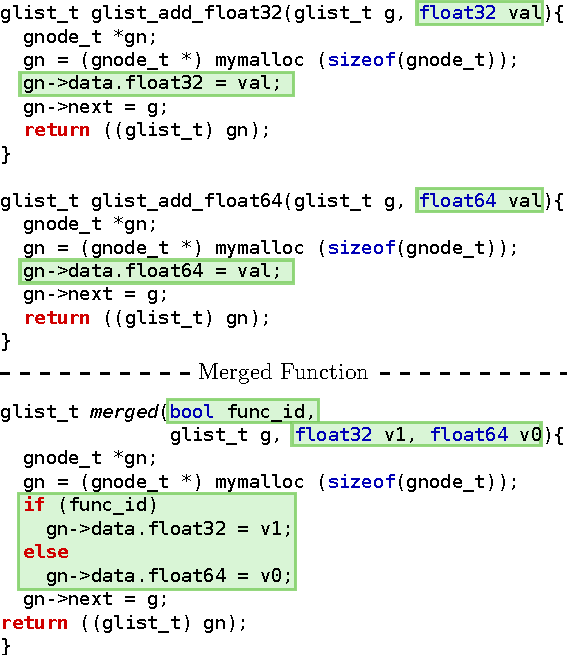
\includegraphics[width=.95\linewidth]{figs/sphinx-example.pdf}
  \caption{Example of two functions with different parameters that could be merged, as shown at the bottom.
           We highlight where they differ.}
  \label{fig:sphinx-example}
\end{figure}

Figure~\ref{fig:sphinx-example} shows two functions from the \texttt{482.sphinx3}. Although these two functions seem identical, their
function arguments are of different types, namely, \textit{float32} and \textit{float64}. In the diagram, we highlight the segments where
the data operations differ from each other. None of the the existing function-merging techniques would merge these two functions, as they
all require both functions to have exactly the same list of parameters, with the same types and in the same order. As shown at the bottom
of Figure~\ref{fig:sphinx-example}, these functions can be merged using two strategies. Firstly, we can expand the function argument list
to include the two parameters of different types. Then, we use a function identifier, \texttt{func\_id}, to indicate which of the two
functions is called. Function merging reduces the total number of machine instructions of the two functions by 18\%.

%If we compile all three functions, we can see that the each one of the two original functions have 14 machine instructions, while the merged function has 23 machine instructions.
%This represents a reduction of 18\% in the total number of instructions.
%However, the proposed optimization is able to merge them as shown at the bottom of Figure~\ref{fig:sphinx-example}. First, we merge both lists of parameters,
%adding an extra parameter used as an identifier to distinguish between the functions. Then, we guard the execution of the instructions that
%are unique to one of the functions using the function identifier. \fixme{ZW: Perhaps not talking about our technique here, but how much
%code reduction we can have by merging these two functions. We then use this to motivate the need of our technique.}

\begin{figure}[t!]
  \centering
  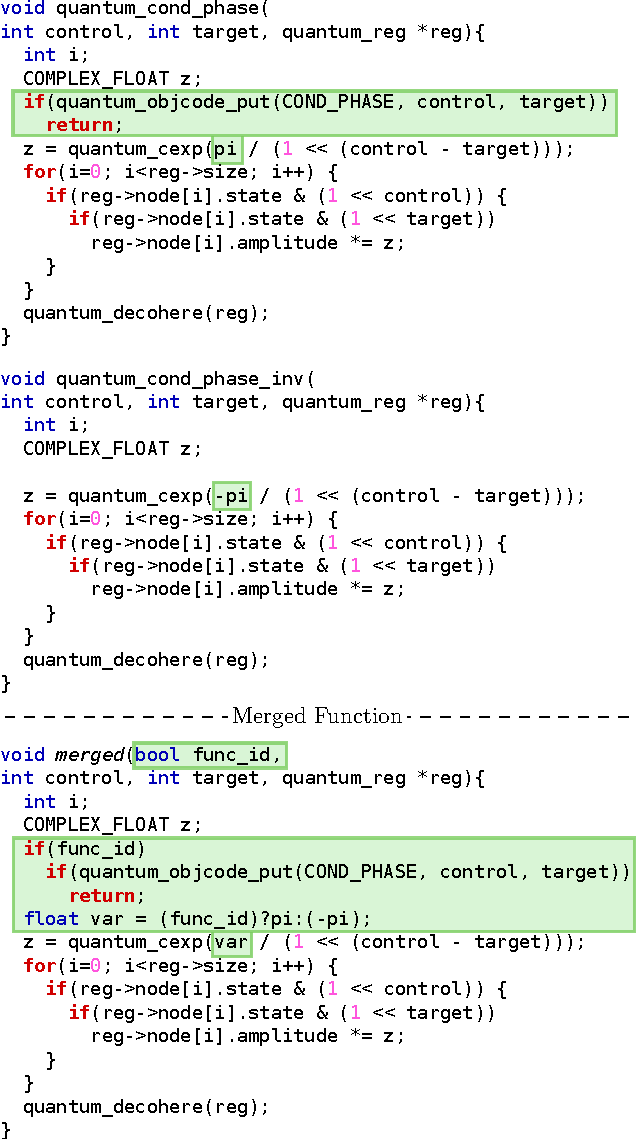
\includegraphics[width=\linewidth]{figs/libquantum-example.pdf}
  \caption{Example of two functions with different CFGs that could be merged, as shown at the bottom.
           We highlight where they differ.}
  \label{fig:libquantum-example}
\end{figure}


Figure~\ref{fig:libquantum-example} gives another two functions extracted from \texttt{462.libquantum}. Although these two functions have
the same signature, i.e., the same return type and list of parameters, they differ in some parts, including their CFGs. None of the
existing techniques can merge the two functions because of the difference in the CFGs. As shown at the bottom of
Figure~\ref{fig:libquantum-example}, these two functions in fact can be merged by simply using a function identifier, \texttt{func\_id}.
Function merging reduces the total number of machine instructions of the two functions by 23\%.

%The existing techniques are unable to merge them due mainly to the structural differences in their CFGs, as we have described in
%Section~\ref{sec:background}. Similar to the previous example, we could merge these two functions, as shown at the bottom of
%Figure~\ref{fig:libquantum-example}. Again, this can be done by using a function identifier. Inspecting the compiled assembly of all three
%functions, we can see a reduction of 27\% in the total number of machine instructions.
%%Similar to the previous example, the proposed optimization is also able to merge these two
%%functions, as shown at the bottom of Figure~\ref{fig:libquantum-example}. Basically, we guard the execution of the code that are unique to
%%one of the functions using the function identifier added to the list of parameters. \fixme{ZW: Again, here we need to give the intuition on
%%why we can merge them and what's the benefit for doing so. I think we should avoid talking about our technique here because at this point
%%the reviewer won't understand how our technique works.}
%=======
%Figure~\ref{fig:libquantum-example} shows two complete functions extracted from the SPEC CPU2006 \texttt{462.libquantum} benchmark.
%Although these two functions have the same signature, i.e., the same return type and list of parameters, they differ in some parts,
%including their CFGs. The existing techniques are unable to merge them due mainly to the structural differences in their CFGs, as we have
%described in Section~\ref{sec:background}.
%Similar to the previous example, we could merge these two functions, as shown at the bottom of Figure~\ref{fig:libquantum-example}. Basically, we just need to guard the execution of the code that is unique to
%one of the functions using the function identifier added to the list of parameters.
%Inspecting the compiled assembly of all three functions, we can see a reduction of 27\% in the total number of machine instructions.
%%Similar to the previous example, the proposed optimization is also able to merge these two
%%functions, as shown at the bottom of Figure~\ref{fig:libquantum-example}. Basically, we guard the execution of the code that are unique to
%%one of the functions using the function identifier added to the list of parameters. \fixme{ZW: Again, here we need to give the intuition on
%%why we can merge them and what's the benefit for doing so. I think we should avoid talking about our technique here because at this point
%%the reviewer won't understand how our technique works.}
%>>>>>>> e85b1a68ed569a46dd18b4379769346de63fc8f8


These examples show that the state-of-the-art function merging methods impose over-restricted constraints on the code structures, and thus
miss massive opportunities. Our work aims to develop a better approach to lift the constraints to merge similar code of any two arbitrary
functions.

\section{Our Approach} \label{sec:fm}

In this section, we describe our proposed function-merging technique, and how it is able to solve the motivating examples as one would expect. Contrary to all existing techniques, ours is able to merge any two arbitrary functions.
For this reason, we also propose a profitability cost model to decide when it is beneficial to merge two functions (see Section~\ref{sec:profit-model}).
If the two functions are equivalent, i.e., identical, then they can be completely merged into a single function.
However, if the two functions differ at any point, an extra parameter is required so that the caller is able to select the correct function.
%The two functions can differ in any possible way, including their list of parameters or return types.
If the lists of parameters are different, we can merge them so that we are able to uniquely represent all parameters from both functions. If the return types are
different, we can use an aggregate type to return values of both types or return just the non-void type if the other one is void.
%\fixme{ZW: Should refer to the motivation example here.}
%However, in our current implementation, the only restriction is that both
%functions must have equivalent return types or one of them must be \textit{void}.

Intuitively, when we are manually merging two functions, in a textual format, we try to visualize them side by side, identifying the equivalent segments of code and the non-equivalent ones. Then, we use this understanding to create the merged function.
In this paper, we propose a technique that follows this intuitive principle.
In the core of our technique lies a sequence alignment algorithm, which is responsible for arranging the code in segments that are either equivalent or non-equivalent.

\begin{figure}[t!]
  \centering
  %\vspace{-1ex}
  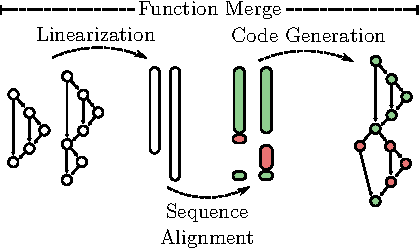
\includegraphics[width=0.85\linewidth]{figs/func-merge-overview.pdf}
  \caption{Overview of our function-merging technique.}
  \label{fig:func-merge-overview}
  %\vspace{-1ex}
\end{figure}

The proposed technique consists of three major steps, as depicted in
Figure~\ref{fig:func-merge-overview}.
First, we linearize each function, representing the CFG as a sequence of
labels and instructions.
The second step consists in applying a sequence alignment algorithm, borrowed
from bioinformatics, which identifies regions of similarity between sequences.
The sequence alignment algorithm allows us to arrange two linearized functions
into segments that are equivalent between the two functions and segments where
they differ from one another.
The final step performs the code generation, actually merging the two functions
into a single function based on the aligned sequences.
Aligned segments with equivalent code are merged, avoiding redundancy, %redundant code,
and the remaining segments where the two functions differ have their code guarded by a function identifier. At this point, we also create a
merged list of parameters where parameters of the same type are shared between the functions, without necessarily keeping their original
order. This new function can then be used to replace the original functions, as they are semantically equivalent, given the appropriate
function-identifier parameter. \fixme{ZW: It is weird sequence alignment is introduced here. We need to explain why using sequence
alignment.}

\subsection{Linearization}

\begin{figure}[b]
  \centering
  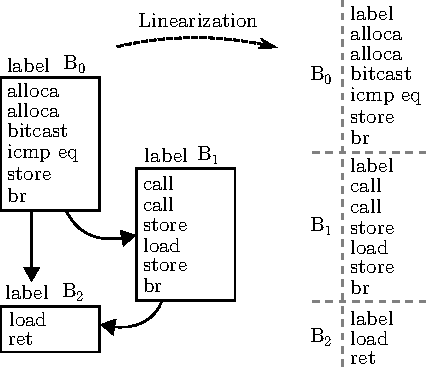
\includegraphics[width=0.7\linewidth]{figs/linearization-example.pdf}
  \caption{An example of the linearization of a CFG.}
  \label{fig:linearization-example}
\end{figure}

The \textit{linearization}\footnote{Although linearization of CFGs
usually refers to a predicated representation, % resulting from an if-conversion,
in this paper, we refer to a simpler definition.} is a key step for enabling the
use of sequence alignment.
It consits in specifying an ordering of the basic blocks based on a traversal
of the CFG and then producing a sequence of labels and instructions, similar to a textual representation of the function.
All instructions from a given basic block must appear right after the label of that basic block, besides maintaining the same order among them.
However, the exact ordering chosen for the basic blocks will not compromise the correctness of the results but it can have an impact on the quality of the merge operation.
Figure~\ref{fig:linearization-example} shows a simplified example of the linearization of the CFG of a function extracted from the \text{400.perlbench} benchmark in SPEC CPU2006.

%Although this operation is trivial, the specific ordering of the basic blocks
%chosen can have an impact on the merging operation.

%For the linearization, we assume that every basic block has an entry label and
%a terminator instruction which refers explicitly to the successor basic blocks,
%if there are successors.
%This is true for most IRs, such as the LLVM IR, or can be easily adapted.

In our implementation, the linearization uses a reverse post-order~(RPO) of the
basic blocks, following a canonical ordering of the successors.
%, e.g., \textit{true} branches before \textit{false} ones.
%Figure~\ref{fig:branch-linearization} shows an example of the linearization
%using the canonical RPO.
%The RPO guarantees that the linearization starts with the entry basic block and then proceeds favoring definitions before uses, except in the presence of loops.
Although the specifc ordering produced by the canonical linearization may not be optimal,
in general it shows good results, as it is also common practice for compilers to rely on prior canonicalizations, e.g., canonical loops, canonical induction variables, canonical reassociation, etc.~\cite{briggs94,liu96}.
By contrast, if, instead, we use an RPO linearization with a uniformly randomized ordering of the successor basic
blocks, the final code-size reduction of the function-merging optimization can deteriorate by 10\% for individual benchmarks.
%Note that our decision for using the canonical RPO is purely pragmatic and other orderings of the basic blocks could also be used, as long as it produces a sequence of labels followed by instructions.

%\begin{figure}[h]
%  \centering
%  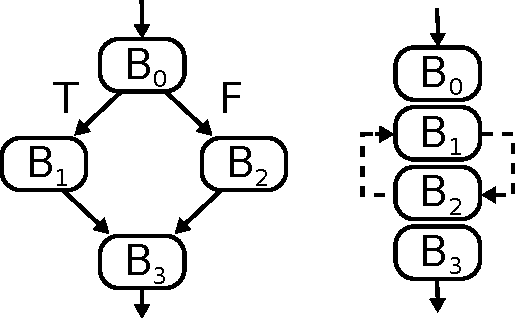
\includegraphics[width=0.6\linewidth]{figs/branch-linearization.pdf}
%  \caption{Linearization using a canonical reverse post-order.
%           The dashed arrows show where a randomized ordering could change the
%           linearization.}
%  \label{fig:branch-linearization}
%\end{figure}

\subsection{Sequence Alignment}

When merging two functions, the goal is to identify which segments of code
are equivalent, and therefore can be merged, and which ones are different.
%and labels that can be merged and which ones need to be selected based on the
%actual function being executed.
To avoid breaking the semantics of the original program, we also need to
maintain the ordering of the instructions for each one of the functions.

To this end, after linearization, we reduce the problem of merging functions
to the problem of \textit{sequence alignment}. %~\cite{carrillo88,wang94}.
%After linearization, the problem of merging two functions can be reduced to the
%\textit{sequence alignment} problem~\cite{carrillo88,wang94}, which is itself
%closely related to finding the
%\textit{longest common subsequence}~\cite{hirschberg75,maier78}.
Sequence alignment is an important technique to many areas of science,
most notably in molecular biology~\cite{needleman70,smith81,carrillo88,wang94}
where, for example, it is used for identifying homologous subsequences of amino
acid in proteins.
Figure~\ref{fig:opcode-align} shows an example of the sequence alignment
between two linearized functions extracted from the \text{400.perlbench} benchmark,
including the one used in Figure~\ref{fig:linearization-example}.

Formally, sequence alignment can be defined as follows:
For a given alphabet $\alpha$, a sequence $S$ of $k$ characters is a subset of
$\alpha^k$, i.e., $S = (a_1, \ldots a_k)$.
Let $S_1, \ldots, S_m$ be a set of sequences, possibly of different lengths but
all derived from the same alphabet $\alpha$, where
$S_i = (a_1^{(i)}, \ldots, a_{k_1}^{(i)})$, for all $i\in\{1,\ldots,m\}$.
%\begin{equation*}
%\begin{align*}
%S_1 = (a_1^{(1)}, \ldots, a_{k_1}^{(1)})\\
%\dots\\
%S_m = (a_1^{(m)}, \ldots, a_{k_m}^{(m)})
%\end{align*}
%\end{equation*}
Consider an extended alphabet that includes the \textit{blank} character ``$-$'',
i.e., $\beta = \alpha \cup \{-\}$.
An alignment of the $m$ sequences, $S_1, \ldots, S_m$, is another set of sequences,
$\bar{S}_1, \ldots, \bar{S}_m$, such that each sequence $\bar{S}_i$ is obtained
from $S_i$ by inserting blanks in positions where some of the other sequences
have non-blank and possibly equivalent characters, for a given equivalence relation.
All sequences $\bar{S}_i$ in the alignment set have the same length $l$, where
$\max\{k_1,\ldots,k_m\} \leq l \leq k_1 + \cdots + k_m$.
Moreover, $\forall i\in\{1,\ldots, m\}$, $\bar{S}_i = (b_1^{(i)},\ldots,b_l^{(i)})$,
there are increasing functions $v_i: \{1,\ldots,k_i\} \to \{1,\ldots,l\}$, such that:
\begin{itemize}[noitemsep,topsep=0pt]
\item $b_{v_i(j)}^{(i)} = a_j^{(i)}$, for every $j \in \{1,\ldots,k_i\}$;
\item any position $j$ not mapped by the function $v_i$, i.e.,
for all $j \in \{1,\ldots,l\}\setminus \textrm{Im} v_i$,
then $b_j^{(i)}$ is a blank character.
\end{itemize}
Finally, for all $j\in\{1,\ldots,l\}$, there is at least one value of $i$ for
which $b_j^{(i)}$ is not a blank character.
%and for any pair of sequences that have a non-blank character at position $j$,
%these characters are equivalent.
Note that two aligned sequences may contain both non-blank and non-equivalent
characters at any given position, in which case it contains a mismatch.

\begin{figure}[t]
  \centering
  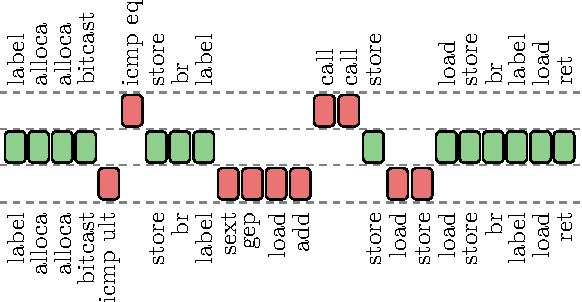
\includegraphics[width=0.75\linewidth]{figs/opcode-align.pdf}
  %\caption{An example of a sequence alignment between two real functions extracted from the \text{400.perlbench} benchmark.}
  \caption{The sequence alignment between two functions, identifying the equivalent segments of code (green in the center) and the non-equivalent ones (red at the sides).}
  \label{fig:opcode-align}
\end{figure}

Specifically for function-merging, we are concerned with the alphabet
consisting of all possible typed instructions and labels.
Every linearized function represents a sequence derived from this alphabet.
We explain the equivalence relation used for this alphabet in the next section.
Although we only consider pair-wise alignments, the technique would also work
for multi-sequences.

%We describe the equivalence relation between two predicated values in two
%separate cases, namely, the equivalence between instructions and the
%equivalence between labels.
%Labels are always considered equivalent.
%Two instructions are equivalent if their opcode are semantically equivalent,
%but not necessarily the same, and they both have types that can be bitcasted in
%a losslessly way from on to the other.
%This also includes making sure that there is no conflict regarding memory
%alignment when handling pointers.
%No additional restriction is imposed on the operands of the two instructions
%being compared for equivalence.
%Whenever two operands cannot be statically proved to represent the same value,
%a select instruction can be used to distinguish between the execution of two
%functions being merged.
%For function calls, the type equivalence requires that both instructions have
%identical function types, i.e., both called functions must have an identical
%return type and an identical list of parameter types.

There is a vast literature on algorithms for performing sequence alignment,
especially in the context of molecular biology.
These algorithms range from optimal algorithms based on dynamic programming to
probabilistic models that do not guarantee
optimality~\cite{needleman70,smith81,carrillo88,hickey11}.
In this paper, we use the Needleman-Wunsh algorithm~\cite{needleman70}.
This algorithm is based on dynamic programming and consists of two main steps.
First, it builds a \textit{similarity matrix}, based on a scoring scheme, which
assigns weights for matches, mismatches, and \textit{gaps} (blank characters).
Afterwards, a backward traversal is performed on the similarity matrix, in order
to reconstruct the final alignment by maximizing the total score.
We use a standard scoring scheme for the Needleman-Wunsh algorithm that rewards
matches and equally penalizes mismatches and gaps.

%\todo{Remove this paragraph.}
%When producing the final aligned sequence, there may be several possible optimal
%alignments.
%However, different aligned sequences can affect the code generation in different
%ways that may be both beneficial or undesirable.
%For this reason, we prioritize alignments that tend to group the blank
%characters together, avoiding to frequently alternate between the two sequences
%during long segments of mismatches and gaps.
%For example, note that in Figure~\ref{fig:opcode-align}, the red blocks, for
%a particular sequence, tend to be grouped together.

\subsection{Equivalence Relation}

In order to merge functions we first need to define what makes two pieces of
code equivalent and therefore mergeable.
In this section, we describe how we define the equivalence relation between values in two
separate cases, namely, the equivalence between instructions and the
equivalence between labels.

Labels can represent both normal basic blocks and landing blocks, which are used
in exception handling code.
Labels of normal basic blocks are always considered equivalent but
landing blocks must have identical landing-pad instructions.
We describe exception handling code in more detail in the next section.

Two instructions are equivalent if: $(1)$ their opcodes are semantically
equivalent, but not necessarily the same; $(2)$ they both have equivalent types;
and $(3)$ they have pairwise operands with equivalent types.
Types are considered equivalent if they can be bitcasted in a lossless way
from one to the other.
It is also important to make sure that there is no conflict regarding memory
alignment when handling pointers.
No additional restriction is imposed on the operands of the two instructions
being compared for equivalence.
Whenever two operands cannot be statically proved to represent the same value,
a select instruction is used to ensure that the correct value will be used in
the computation.
%distinguish between the execution of two functions being merged.
For function calls, the type equivalence requires that both instructions have
identical function types, i.e., both called functions must have identical
return types and identical list of parameters.

\subsubsection{Handling Exception Handling Code}

In this section, we describe restrictions imposed by exception handling code and
their equivalence relation.
Most modern compilers implement the zero-cost Itanium ABI for exception
handling~\cite{dinechin00}, including GCC and LLVM, sometimes called the
\textit{landing-pad} model.
In this model, landing-pad instructions are used to encode which action is taken
when an exception has been thrown.
%The type of equivalent landing-pad instructions must be identical as its value
%is crucial in deciding what action to take when the landing block is entered,
%and corresponds to the return value of the personality function, which must also
%be identical for the two functions being merged.

The invoke instruction co-operates tightly with its landing block, i.e., the
basic block pointed by the exception branch of an invoke instruction.
The landing block must have a landing-pad instruction as its first non-$\phi$
instruction.
Given this restriction, two equivalent invoke instructions must also have
landing blocks with identical landing-pad instructions.
This restriction can be easily checked since the landing-pad instruction is
always the first instruction in a landing block.

Landing blocks are responsible for handling all catch clauses covering the
particular call site, in the high-level code.
All clauses are defined by the landing-pad instruction, which encodes the list of
all exception and cleanup handlers.
Landing-pad instructions are equivalent if they have exactly the same type and
also encode identical lists of exception and cleanup handlers.

%The return value of the landing-pad instruction is crucial in deciding what
%action to take when the landing block is entered, and corresponds to the return
%value of the personality function.

%In other words, when the unwinder executes the personality function (which
%is part of the language runtime), it stores its return value, and provides this return value in the result of the landing-pad
%instruction. Since the personality function has access to the part of the unwind tables generated from the landing-pad
%instruction, it can communicate information encoded in the unwind table to the landing block itself. In the libc++ runtime,
%the personality function returns a tuple consisting of a pointer to the exception object itself, and a “handler switch value”, an
%integer which corresponds to the index of a relevant “catch” clause of the landing-pad instruction, or a special value (−1)
%when no catch clauses match but a cleanup needs to be performed.

%The LLVM IR generated for the landing block then checks the handler switch value computed by the personality function,
%and transfers control to a cleanup or handler block accordingly.

%Finally, if the selected handler is a cleanup handler, the
%exception propagation (stack unwinding) needs to be resumed after the cleanup is done. This is achieved by the resume
%instruction, which expects as a parameter the same value that was returned by the corresponding landing-pad instruction
%which interrupted the exception propagation.
%Interestingly, there are no LLVM instructions for raising (throwing) exceptions. This is left entirely in the management
%of the language runtime, which needs to closely co-operate with the stack unwinding library anyway (the interface of the
%personality function is mandated by the stack unwinder).

\subsection{Code Generation}

The code generation phase is responsible for producing a new function from the
result of the sequence alignment.
This phase has three main concerns: merging the two lists of parameters;
%from both functions;
generating the necessary select instructions in order to
use the appropriate operands in merged instructions;
%distinguish between the execution of the appropriate function;
constructing the CFG of the merged function.

%\subsubsection{Merged Parameters}

If the lists of parameters are different, we can merge them so that we are able
to uniquely represent all parameters from both functions.

The merged list of parameters must contain exactly one parameter that uniquely
represents each one of the parameters from both functions, without necessarily
maintaining the same order.
%The merged list of parameters must be able to represent all parameters from
%both functions, where the each individual parameter in the merged list of
%parameters can represent at most one parameter of both functions.
An extra binary parameter, called the function identifier, is also added to the
merged list of parameters.
This extra parameter is required to distinguish between the two merged functions.
Figure~\ref{fig:merged-params} depicts how we merge the list of parameters of
two functions.
First, we create the binary parameter that represents the function identifier,
one of the functions will be identified by the value \textit{true} and the other
by value \textit{false}.
We then add all the parameters of one of the functions to the new list of
parameters.
Finally, for each parameter of the second function, we either reuse an existing
and available parameter of identical type from the first function or we add a
new parameter.
We then keep track of the mapping between the lists of parameters of the
original functions and the merged function so that, later, we are able to
replace the function calls.
When replacing the function calls to the new merged function, parameters that
are not used by the original function being called will receive undefined values.
%For this reason, it is important to be careful when merging the two functions
%in order to avoid creating unsafe computation on undefined values, which
%results in undefined behavior.

The reuse of parameters between the two merged functions provides the following
benefits:
%(1) it allows for a simpler function call, with fewer values to pass to the
%called function, reducing code size;
%(2) similarly, it reduces the frame of the merged function;
(1) it reduces the overheads concerning function call abstractions, such as,
reducing the number of values required to be communicated between functions.
(2) if the reused parameters have similar usage by both functions, it may reduce
the number of select instructions that are needed to distinguish between the
merged functions.

\begin{figure}[h]
  \centering
  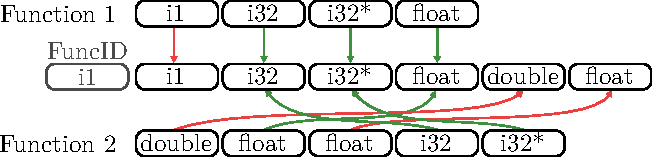
\includegraphics[width=0.9\linewidth]{figs/merged-params.pdf}
  \caption{Example of a merge operation on the list of parameters of two functions.}
  \label{fig:merged-params}
\end{figure}


When multiple available parameters of one function have the same type as a given
parameter from the other function, we choose the one that minimizes the number
%of select instructions by analyzing all pairs of matching instructions in the
%aligned sequence that contain the parameters as operands.
of select instructions.
%We are able to find pairs of parameters that minimize the number of selects by
The pairs of parameters that minimize the number of selects can be found by
analyzing all pairs of matching instructions, in the aligned sequence, that
contain the corresponding parameters as operands.
Experiments show that maximizing the matching of parameters, compared to never
%merging them, improves the average code-size reduction in about 1\%, with
%improvements in individual benchmarks of up to 7\%.
merging them, improves code-size reduction of individual benchmarks by up to 7\%.


%\subsubsection{Control-Flow Graph Reconstruction}

After generating the merged list of parameters, we perform a code generation
to produce the CFG of the merged function in two passes over the aligned
sequence.
The first pass creates the basic blocks and instructions.
The second assigns the correct operands to the instructions, which also connects
the basic blocks.
A two-passes approach is required in order to handle loops, due to cyclic data
dependencies.
%Listing~\ref{lst:CodeGen} presents the pseudocode for the code generation.

%\begin{myfloat}[h]
%  \begin{lstlisting}[caption={Pseudocode for the code generation. \todo{simplify.}}, label={lst:CodeGen}]
%CodeGen(Sequence, Function) {
% CFG = Function.NewCFG()
% VMap = Mapping of values to values
% MergedBB = null
% TailBB = Mapping of labels to labels
% //first pass: create CFG and instructions
% for each Entry in Sequence:
%   if Entry is a match:
%      if Entry is of labels:
%         BBLabel = CFG.NewBlock()
%         ValMap[Entry[0]] = BBLabel
%         ValMap[Entry[1]] = BBLabel
%         if Entry has landing-pad:
%           create landing-pad for BBLabel
%         MergedBB = BBLabel
%      if Entry is of instructions:
%         I0, I1 = Entry[0], Entry[1]
%         if MergedBB is null:
%           MergedBB = G.addBasicBlock()
%           TailBB[I0.getBlock()].addBranch(MergedBB)
%           TailBB[I1.getBlock()].addBranch(MergedBB)
%         add cloned instruction to MergedBB
%         if Entry is terminator instruction:
%           MergedBB = null
%   else:
%      if MergedBB not null:
%        branch to two new basic blocks
%        add new basic blocks to TailBB
%        MergedBB = null
%
%      if Entry is a label:
%        BBLabel = G.NewBlock()
%        ValMap[Entry] = BBLabel
%      if Entry is an instruction:
%        BB = TailBB[Entry.getBlock()]
%        add cloned instruction to the BB
%
% //second pass: update operands
% for each Entry in Sequence:
%   if Entry is a match:
%      if Entry is of instructions:
%         I0, I1 = Entry[0], Entry[1]
%         I = ValMap[I0]
%
%         for each (Op0, Op1) in I0 and I1:
%           Op0Val = ValMap[Op0]
%           Op1Val = ValMap[Op1]
%           OpVal = Op0Val //assuming equality
%           if ValMap[Op0]!=ValMap[Op1]:
%              OpVal = G.addSelect(Op0Val,Op1Val)
%           update operand of I with OpVal
%   else:
%      if Entry is an instruction:
%        I = ValMap[Entry]
%        update all operands of I using ValMap
%
%}
%  \end{lstlisting}
%\end{myfloat}

First, for each entry in the aligned sequence, we either create a new basic
block for labels or we add a cloned instruction to the appropriate basic
block.
If the label represents a landing block, a landing-pad instruction is also added
to the new basic block.
During this process, we keep a mapping from the instructions and labels in the
original functions to their corresponding values in the new merged function.
This mapping is required to appropriately create the use-definition
chains for the merged function, which is done by pointing the operands of the
instructions to the correct values in the function.
However, at this point, the cloned instructions are created with empty operands,
as we are still creating the complete mapping.

While iterating over the aligned sequence, we also need to create extra basic
blocks and branch instructions in order to maintain the semantics of the
original functions, guarding the execution of instructions that are unique to
one of the functions being merged.
When transitioning from matching instructions or labels to non-matching ones,
we need to branch to new basic blocks based on the function identifier.
This divergent point is used to continue code generation for the contiguous
non-matching segment of the aligned sequence.
When trasitioning back from non-matching segments to a matching segment, we need
to reconnect both divergent points by branching back to a single new basic block
where merged instructions will be added.

The second pass over the aligned sequence is solely responsible for updating
the operands of all the instructions and adding select instructions as necessary.
Select instructions are created when a merged instruction has different operand
values in the original functions, such that the appropriate value needs to be
selected based on the function identifier.
However, if the operands are labels, instead of adding a select instruction,
the operand selection is performed in a control-flow manner, using a new basic
block and a conditional branch based on the function-identifier parameter.
When the two labels represent landing blocks, we hoist the landing-pad
instruction to the new common basic block, converting it to a landing block and
converting the two landing blocks to normal basic blocks.
This is required for the correctness of the landing-pad model.
Additionally, similar to previous work on vectorization~\cite{porpodas18}, we
also exploit commutative instructions in order to maximize similarity.
When assigning operands to commutative instructions, we perform operand
reordering to maximize the number of matching operands and reduce the total
number of select instructions required.

It is important to note that if we are merging two identical functions, no
select or extra branch instruction will be added.
As a result, we can remove the extra parameter that represents the function
identifier.

\section{The Exploration Framework}
\label{sec:framework}

%In this section, we describe our implementation of the function merging
%optimization, which combines the proposed function-merging technique with an
%efficient exploration infrastructure.

In this section, we describe our exploration infrastructure for the 
function merging optimization.
Although the proposed technique is able to merge any two functions, it is not
always profitable to merge them.
In fact, as it is only profitable to merge functions that are sufficiently
similar, for most pairs of functions, merging them increases code size.
Therefore, the main goal of the exploration infrastructure is to efficiently
find pairs of functions that are profitable to merge.

As described in Section~\ref{sec:background}, LLVM's existing function merging
optimization, due to its hard restriction of only merging identical functions,
is able to  efficiently explore which functions to merge by computing a hash
of the functions.
If two functions have the same hash, they are very likely to be identical.
Moreover, merging identical functions is always profitable.
For the proposed function-merging technique, on the other hand, because it is
able to merge any pair of functions, we have a much larger exploration space and
also a more challenging decision problem.

%\subsection{Ranking Infrastructure}

For every function, ideally, we would like to try to merge it with all other
functions and choose the pair that maximizes the reduction in code size.
However, this quadratic exploration over all pairs of functions results in
compilation-time overheads that are usually unacceptable for real-world
scenarios.
In order to avoid the quadratic exploration of all possible merges, we propose
the framework shown in Figure~\ref{fig:func-merge-opt-arch} for the our
optimization.
\begin{figure}[h]
  \centering
  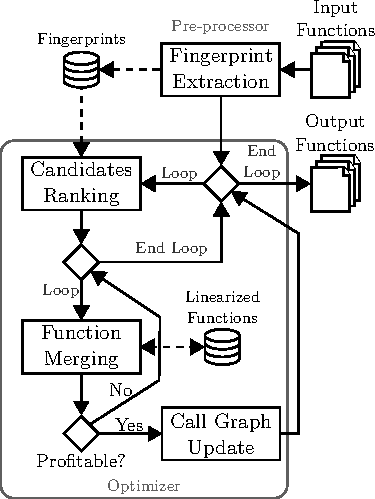
\includegraphics[width=0.65\linewidth]{figs/func-merge-opt-arch.pdf}
  \caption{Overview of our exploration framework.}
  \label{fig:func-merge-opt-arch}
\end{figure}

The proposed framework is based on a light-weight ranking infrastructure that
uses a \textit{fingerprint} of the functions to evaluate their similarity.
It starts by first precomputing and caching the fingerprint of all functions.
The goal of the fingerprint is to allow us to efficiently discard unpromising
pairs of functions so that we perform the more expensive evaluation only on
the topmost similar pairs.
To this end, the fingerprint consists of: $(1)$ map of instruction opcodes to
their frequency in the function; $(2)$ the set of types manipulated by the
function.
While functions can have several thousands of instructions, an IR usually has
just a few tens of opcodes, e.g., the LLVM IR has only about 64 different
opcodes.
This means that the fingerprint needs to store just a small integer array of the
opcode frequencies and a set of types, which allows for an efficient similarty
comparison.

By comparing the opcode frequencies of two functions, we are able to estimate
an upper bound of the merge between these functions, assuming that all
instructions with the same opcode would always result in a match.
This assumption provides an upper bound on the actual number of matches, since
it may be affected by the instruction types and the order they appear in the
linearized functions.
As a way to refine this estimate, we weight this upper bound by the Jaccard
similarity coefficient~\cite{jaccard} of the sets of types, i.e., a
type-similarity ratio between the two functions.
Formally, let $T_1$ and $T_2$ be the set of types of the functions $f_1$ and
$f_2$, respectively.
Therefore, the upper-bound reduction, computed as a ratio, can be defined as
\vspace{-1.5ex}\[
   U\!B(f_1,f_2) = \frac{\sum\limits_{op \in Ops} \min\{freq(op,f_1),freq(op,f_2)\}}{\sum\limits_{op \in Ops} freq(op,f_1)+freq(op,f_2)}
\vspace{-1.5ex}
\]
and the weighted estimate is given by
\vspace{-1.5ex}\[
     s(f_1,f_2) = U\!B(f_1,f_2) \frac{|T_1 \cap T_2|}{|T_1 \cup T_2|}.
\vspace{-1.5ex}
\]
This weighted estimate results in a value in the range $[0,0.5]$,
which encodes a description that favors maximizing both the opcode and type
similarities, while also minimizing their respective differences.
Identical functions will always result in the maximum value of $0.5$.

For each function $f_1$, we use a priority queue to rank the topmost
similar candidates based on their similarity, defined by $s(f_1,f_2)$, for all
other functions $f_2$.
We use an exploration threshold to limit how many top candidates we will
evaluate for any given function.
This cadidate exploration is then performed in a greedy fashion, where the first
candidate that actually results in a profitable merge ends the exploration and
the merge operation is finally commited.

\begin{figure}[h]
  \centering
  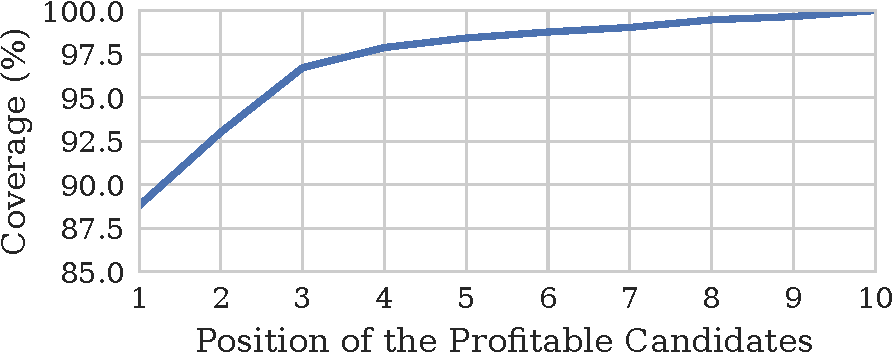
\includegraphics[width=0.8\linewidth]{figs/average-cdf-exploration-threshold.pdf}
  \caption{Average CDF for the exploration threshold and the percentage of merged operations covered.
           89\% of the merge operations happen with the topmost candidate.}
           %A merge operation happens with the topmost candidate in about 89\% of the cases.}
  \label{fig:average-cdf-exploration-threshold}
\end{figure}

Ideally, the profitable candidate will be as close to the top of the rank as
possible.
Figure~\ref{fig:average-cdf-exploration-threshold} shows the cummulative
distribution of the position of the profitable candidates in a top 10 rank.
It shows that about 89\% of the merge operations occurred with the topmost
candidate, where the top 5 covers over 98\% of the profitable candidates.
These results suggest that the proposed fingerprint similarity is able to
accuretly capture the real function similarity, while possibly reducing the
exploration cost by a few orders of magnitudes, depending on the actual number
and size of the functions.

When a profitable candidate is found, then we first replace the body of the two
original functions to a single call to the merged function.
Afterwards, if the original functions can be completely removed, we update the
call graph, replacing the calls to the original functions by calls to the
merged function.
When compiling the whole program, during link-time optimization, we can be more
aggressive when removing the original functions.
However, if the optimization is applied per compilation unit, then extra
conditions must be guaranteed, e.g., the function must not be externally visible
to other compilation units.
Finally, the new function is added to the optimization working list.
Because of this feedback loop, merge operations can also be performed on
functions that resulted from previous merge operations.

\subsection{Profitability Cost Model}\label{sec:profit-model}

After generating the code of the merged function, we need to estimate the
code-size benefit of replacing the original pair of functions by the new merged
function.
In order to estimate the code-size benefit, we first compute the code-size cost
for each instruction in all three functions.
In addition to measuring the difference in size of the merged function, we also
need to take into account all extra costs involved:
$(1)$ for the cases where we need to keep the original functions with a call to
the merged function;
and $(2)$ for the cases where we update the call graph, there might be an extra
cost with a call to the merged function due to the increased number of arguments.

Let $c(f)$ be the code-size cost of a given function $f$, and
$\delta(f_i, f_j)$ represent the extra costs involved when replacing or
updating function $f_i$ with the function $f_j$.
Therefore, given a pair of functions $\{f_1,f_2\}$ and the merged function
$f_{1,2}$, we want to maximize the profit defined as:
\[
  \Delta(\{f_1,f_2\},f_{1,2}) = (c(f_1)+c(f_2)) - (c(f_{1,2}) + \varepsilon)
\]
where $\varepsilon = \delta(f_1, f_{1,2}) + \delta(f_2, f_{1,2})$.
We consider that the merge operation is profitable if $\Delta(\{f_1,f_2\},f_{1,2})>0$.

However, because we are operating on the IR level, one IR instruction does not
necessarily translate to one machine instruction.
Because of that, the profitability is measured with the help of the compiler's
target-spcific cost model.
The actual cost of each instruction comes from querying this compiler's built-in
cost model, which provides a target-dependent cost estimation that approximates
the code-size cost of an IR instruction when lowered to machine instructions.
Our implementation makes use of the code-size costs provided by LLVM's
target-transformation interface (TTI), which is widely used in the decision
%making by most of the LLVM's optimizations.
making of most optimizations.

\section{Evaluation}


In this section, we evaluate the proposed optimization, where we analyze our
improvements on code size reduction, as well as its impact on the program's
performance and compilation-time.



\subsection{Experimental Setup}
We compare our optimization against the state-of-the-art function merging approach of Edler von Koch et al.~\cite{edler14} and LLVM's identical
function merging. In our evaluation, we refer to identical function merging as \textit{Identical}, the state-of-the-art as \textit{SoA}, and our
approach as \textit{FMSA}.

All optimizations are implemented in LLVM v7 and evaluated on the C/C++ SPEC CPU2006~\cite{spec} benchmark suite. We target two different
instruction sets, the Intel x86-64 and the ARM Thumb. Our Intel test bench has a quad-core 3.4~GHz Intel Core i7 CPU with 16~GiB of RAM.
%The operating system is openSUSE 42.2 with Linux kernel version 4.4.27.
The ARM test bench has a Cortex-A53 ARMv8 CPU of 1.4~GHz with 1~GiB of RAM.
%The operating system of the ARM platform is a Raspbian.
We use the Intel platform for compiling for either target. As a result, compilation-time is almost
identical for both targets. Changing the target only affects the behavior of the backend, a very
short part of the pipeline. Because of that, we only report compilation-time overhead results for
one of the targets, the Intel ISA.

\begin{figure*}[t!]
  \centering
  %\subfigure[Intel platform.]{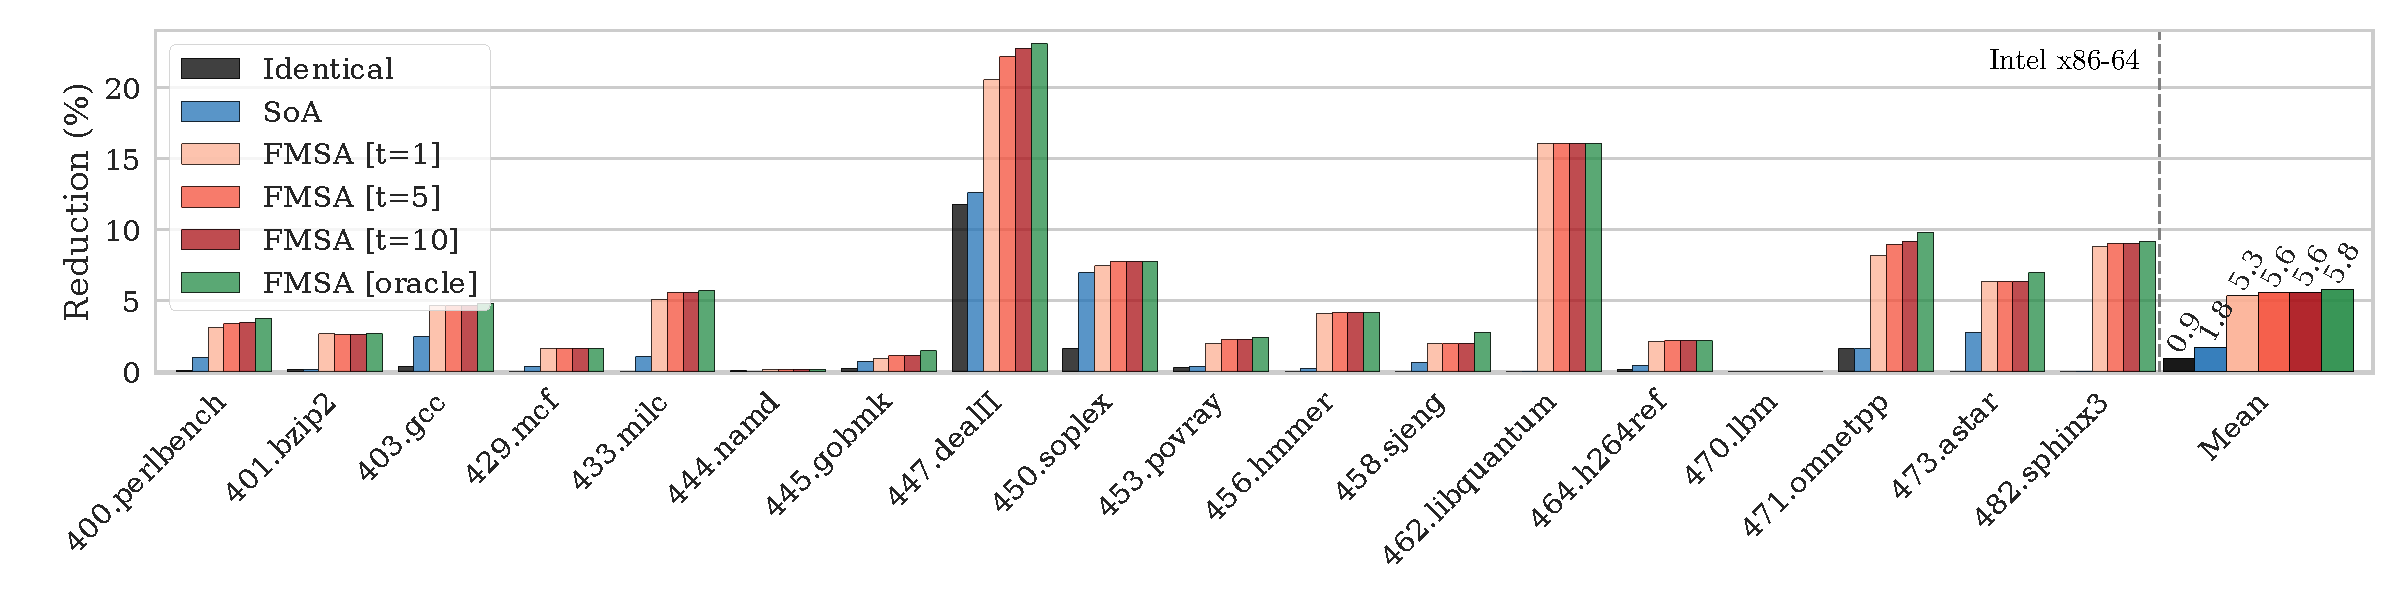
\includegraphics[width=\linewidth]{figs/reduction-obj-intel-label.pdf}}
  %\subfigure[ARM platform.]{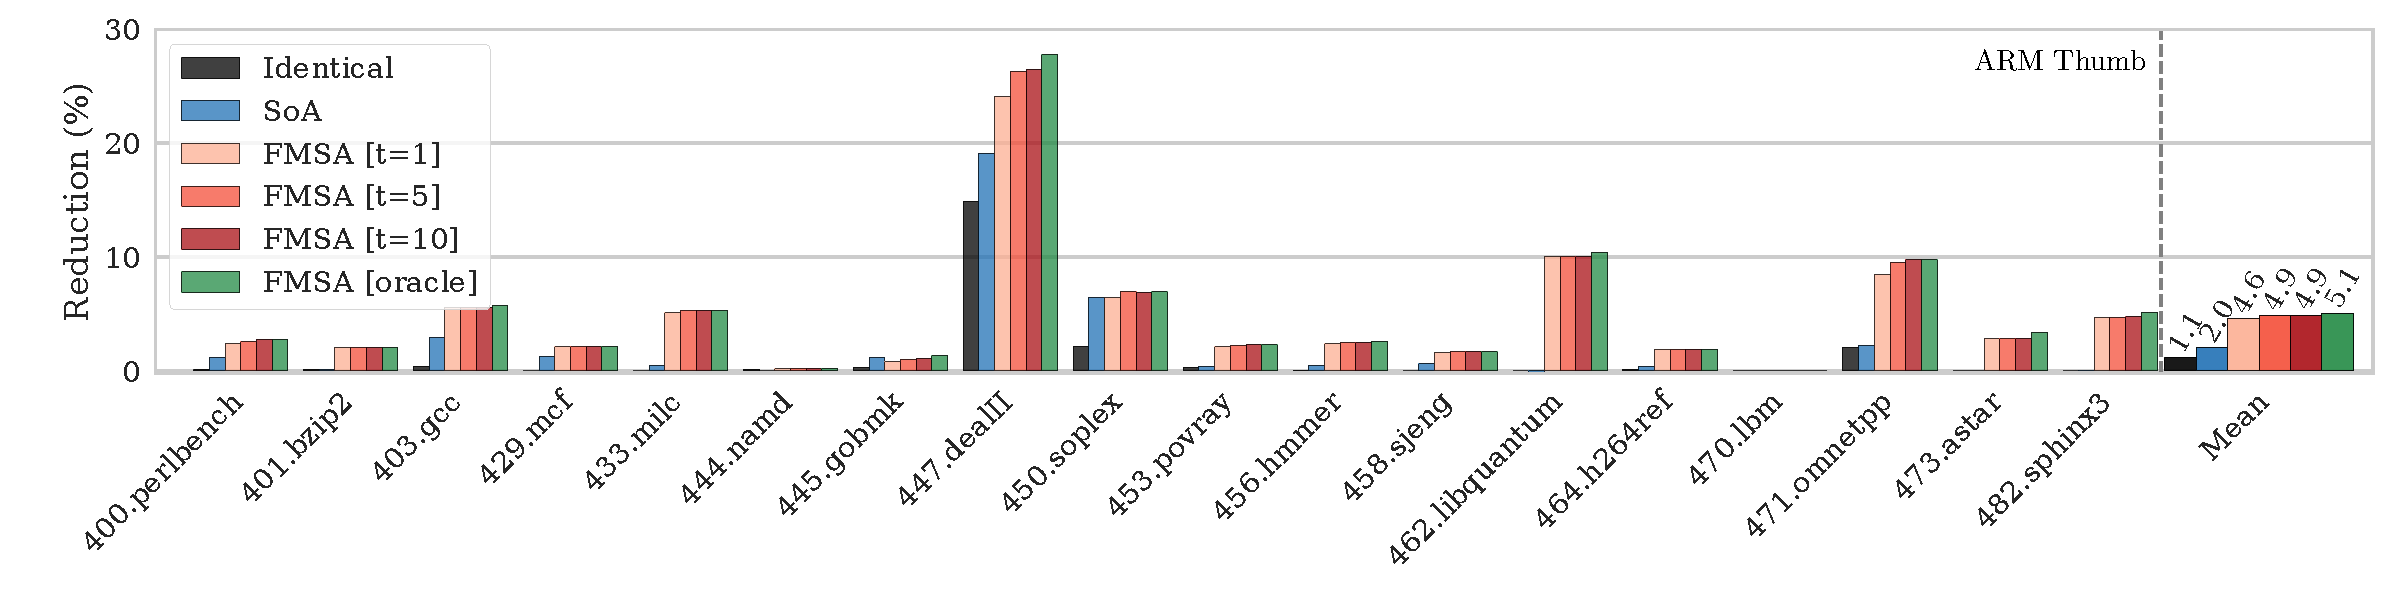
\includegraphics[width=\linewidth]{figs/reduction-obj-arm-label.pdf}}
  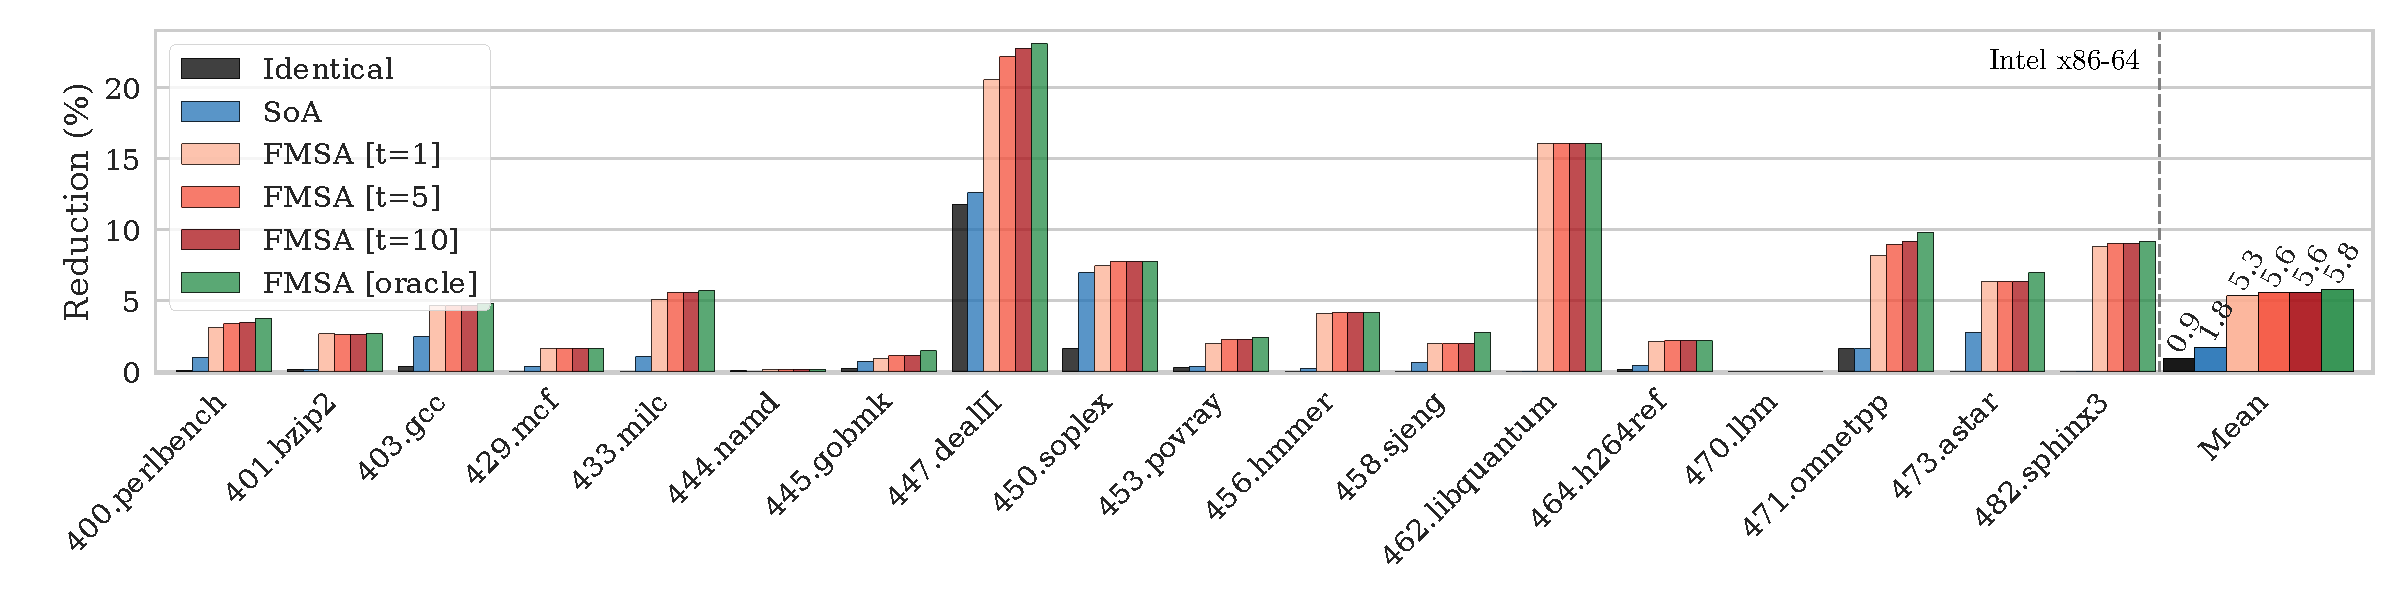
\includegraphics[width=\linewidth]{figs/reduction-obj-intel-label.pdf} \\
  \vspace{-1.8ex}
  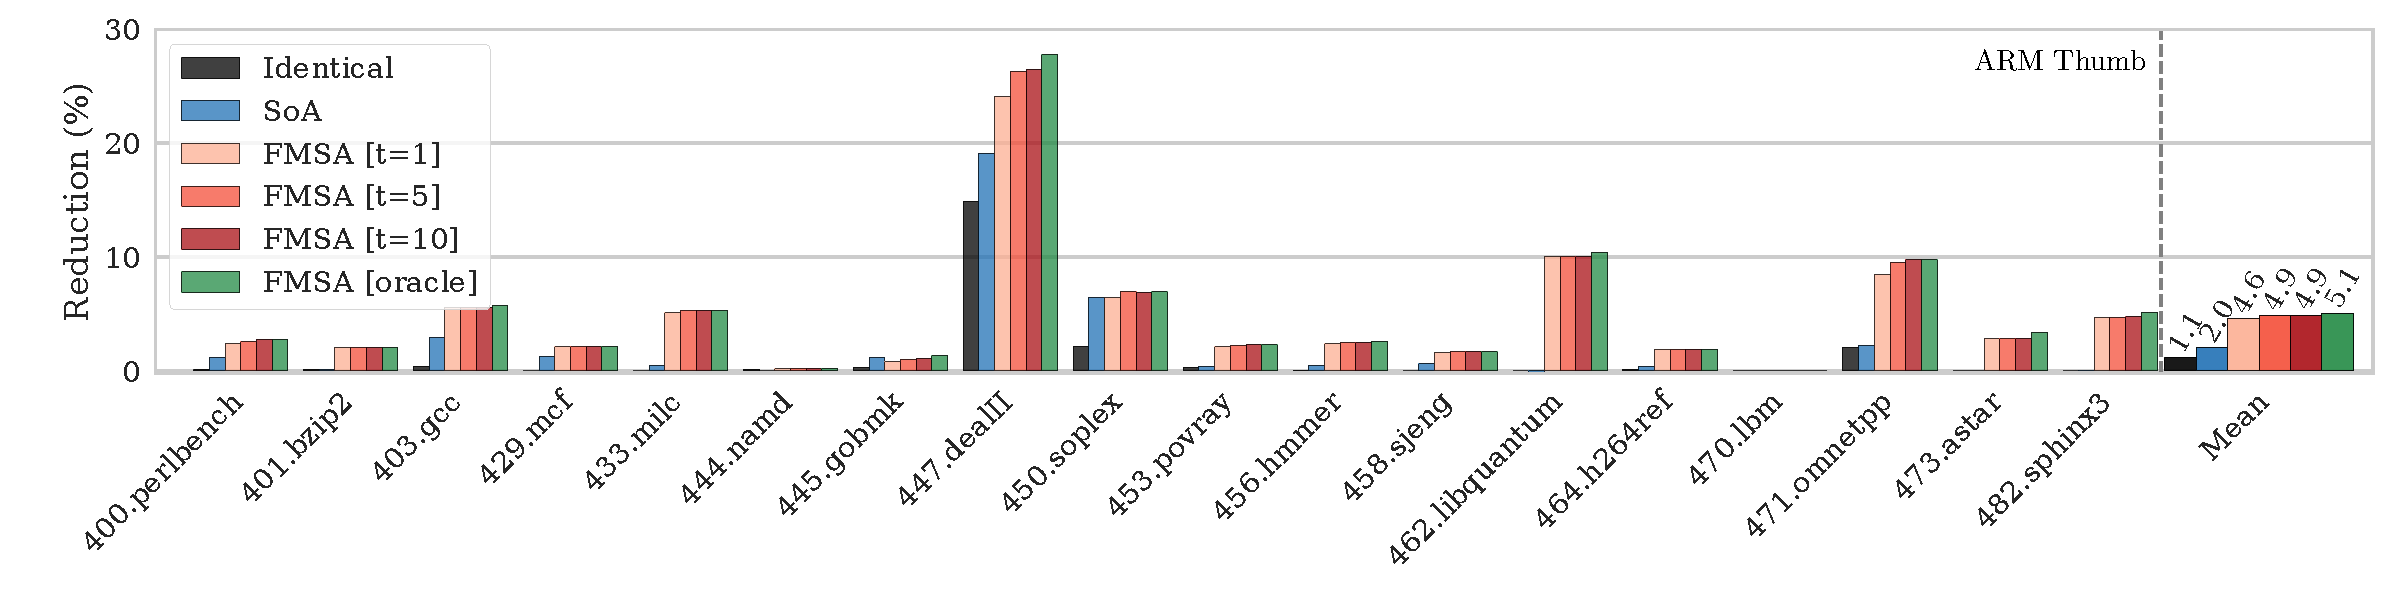
\includegraphics[width=\linewidth]{figs/reduction-obj-arm-label.pdf}
  \vspace{-4ex}
	\caption{Object file size reduction for Intel (top) and ARM (bottom). We evaluate our approach (FMSA) under four different exploration thresholds, which
      control how many potential merging pairs we examine for each function before making a decision. Even for a threshold of one, we outperform the state-of-the-art
	  by 2.9$\times$(Intel) and 2.3$\times$ (ARM).}
  \label{fig:reduction-obj}
\end{figure*}

For the proposed optimization, we vary the exploration threshold (Section~\ref{sec:framework})
and we present the results for a range of threshold values. We also show the results for the oracle exploration strategy, which
instead of using a rank-based greedy approach, merges a function with all candidates and chooses the best one.
%The oracle represents the results assuming a perfect ranking strategy.
%However, the oracle has a very costly quadratic exploration, as explained in
%Section~\ref{sec:framework}.
This oracle is a perfect ranking strategy but is unrealistic. It requires a very costly quadratic exploration, as explained in
Section~\ref{sec:framework}. \fixme{ZW: I suggest we call ``oracle" exhaustive-exploration instead. ``oracle" is often used to refer the
up-bound performance.}



\subsection{Code-Size Reduction}

%\begin{figure*}[th]
%  \centering
%  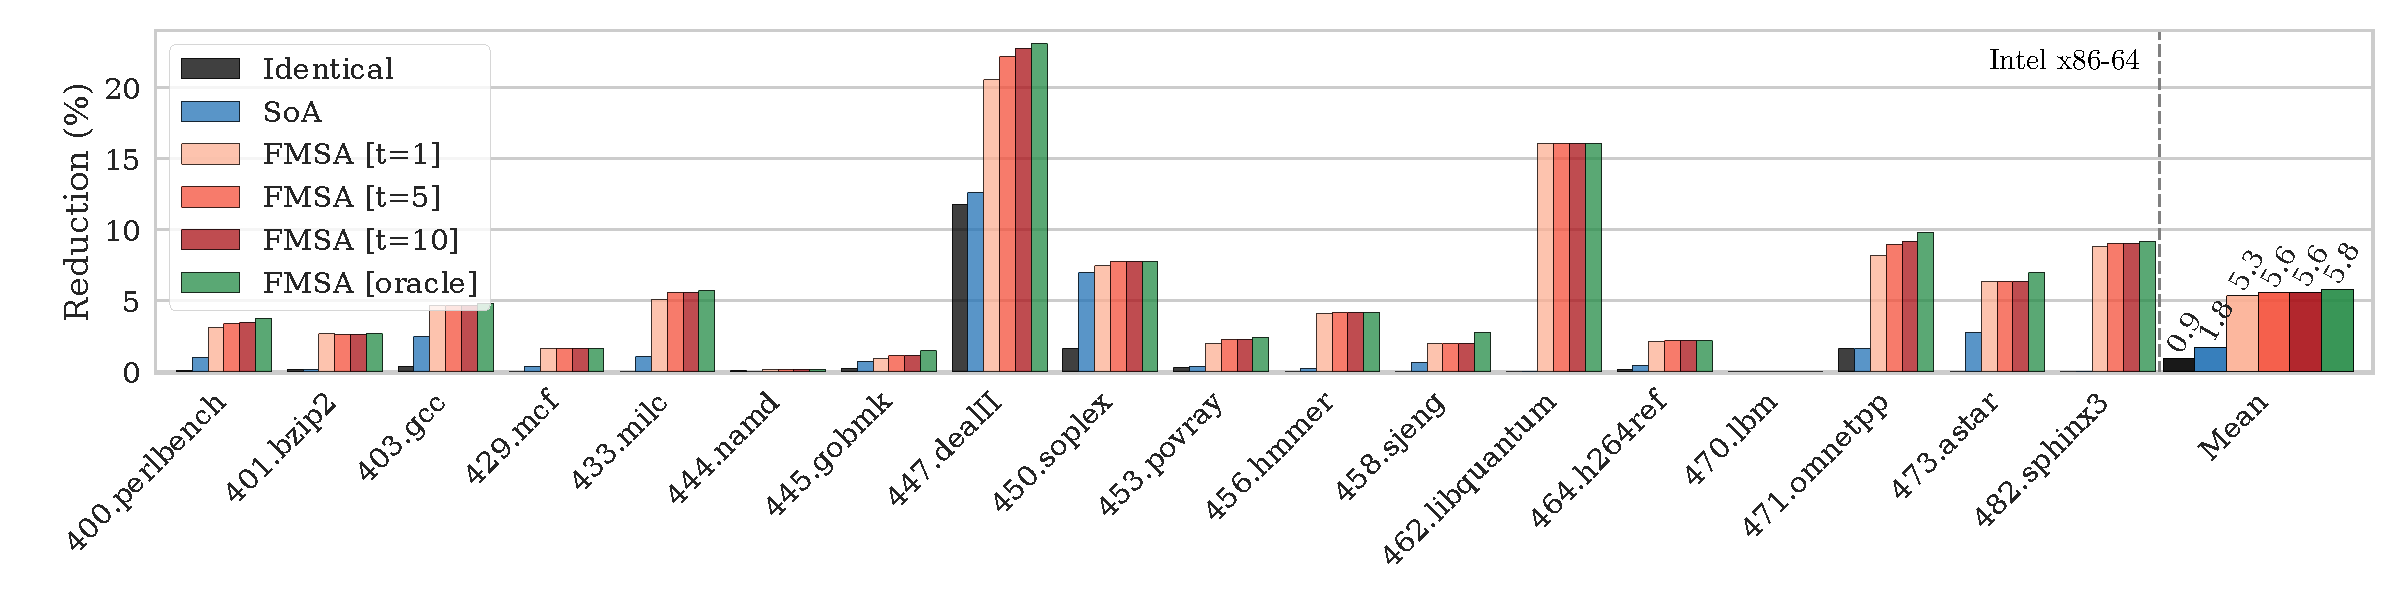
\includegraphics[width=\linewidth]{figs/reduction-obj-intel-label.pdf}
%  \caption{Reduction on the object file for the Intel architecture.}
%  \label{fig:reduction-obj-intel}
%\end{figure*}
%\begin{figure*}[th]
%  \centering
%  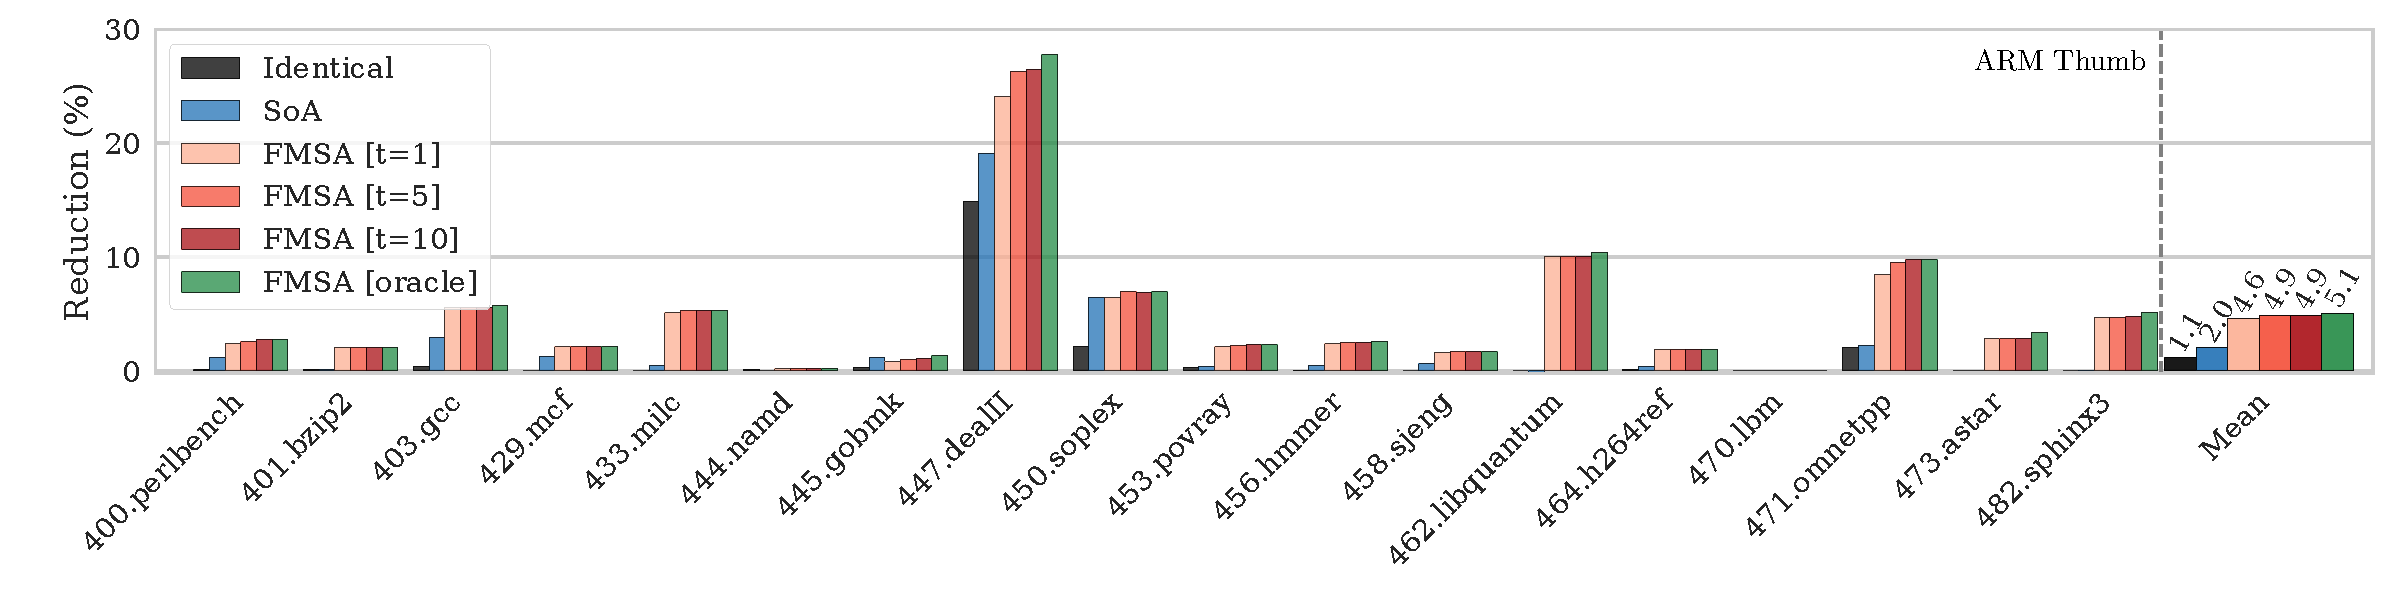
\includegraphics[width=\linewidth]{figs/reduction-obj-arm-label.pdf}
%  \caption{Reduction on the object file for the ARM architecture.}
%  \label{fig:reduction-obj-arm}
%\end{figure*}


Figure~\ref{fig:reduction-obj} reports the code size reduction over the baseline for the linked object. %These results show how much we can improve over the existing techniques, by having a more powerful solution, and how close we
%can get to the oracle with our ranking-based exploration framework.
We observe similar trends of code size reduction on both target architectures. This is expected because the
optimizations are applied at the platform-independent IR level. Changing the target architecture introduces only second order effects,
such as slightly different decisions due to the different cost model (LLVM's TTI) and differences in how the IR is encoded into binary.

Our approach, FMSA, significantly improves over the state-of-the art (SoA). For the Intel platform, FMSA can achieve an average code size
reduction of up to 5.8\% (or 5.3\% with the lowest exploration threshold), while the SoA and Identical had an average reduction of 1.8\% and 0.9\%,
respectively. Similarly, for the ARM platform, FMSA can achieve an average code size reduction of up to 5.1\% (or 4.6\% with the lowest
threshold), while SoA and Identical had an average reduction of 2\% and 1.1\%, respectively. For several of the benchmarks, the
proposed technique achieves impressive code size reduction compared to other merging approaches. Table~\ref{tab:reduction} highlights
some of these results for both platforms. In two cases, \texttt{462.libquantum} and \texttt{482.sphinx3}, the state-of-the-art slightly
increases code size, while FMSA reduces size significantly.  The only case where SOA outperforms FMSA is on the \texttt{445.gobmk}
benchmark on the ARM platform. There are little opportunities for function merging on that benchmark and FSMA misses a few of them.
However, we can easily fix this by increasing the exploration threshold. For exhaustive exploration, FMSA improves over the SoA,
with a code size reduction of 1.33\%. In all other cases, FMSA is always equal or better than all other function-merging optimizations, usually by a significant margin.

\begin{table}[]
\label{tab:reduction}
\centering
\scalebox{0.8}{
\begin{tabular}{lccc}
\toprule
\multicolumn{1}{c}{\textbf{Benchmarks}} & \textbf{Identical} & \textbf{SoA}  & \textbf{FMSA {[}t=1{]}} \\
\midrule
%%%400.perlbench                             & 0.09 / 0.09        & 1.03 / 1.15   & 3.13 / 2.40             \\ \hline
\rowcolor{evencolor} 401.bzip2                                 & 0.15 / 0.16        & 0.15 / 0.16   & 2.67 / 2.09             \\
%%%403.gcc                                   & 0.36 / 0.43        & 2.48 / 2.89   & 4.71 / 5.59             \\ \hline
%%%429.mcf                                   & 0 / 0              & 0.41 / 1.29    & 1.66 / 2.11             \\ \hline
433.milc                                  & 0 / 0              & 1.08 / 0.46   & 5.09 / 5.12             \\
%%%444.namd                                  & 0.10 / 0.14        & 0 / 0         & 0.20 / 0.17             \\ \hline
\rowcolor{evencolor} 447.dealII                                & 11.77 / 14.83      & 12.59 / 19.12 & 20.57 / 24.08           \\
445.gobmk                                 & 0.26 / 0.32        & 0.77 / 1.15   & 0.96 / 0.78             \\
%%%450.soplex                                & 1.62 / 2.16        & 6.99 / 6.47   & 7.46 / 6.48             \\ \hline
\rowcolor{evencolor} 453.povray                                & 0.28 / 0.33        & 0.38 / 0.40   & 2.04 / 2.12             \\
456.hmmer                                 & 0 / 0              & 0.27 / 0.50   & 4.15 / 2.40             \\
%%%458.sjeng                                 & 0 / 0              & 0.63 / 0.63   & 1.97 / 1.62             \\ \hline
\rowcolor{evencolor} 462.libquantum                            & 0 / 0              & -0.07 / -0.17 & 16.08 / 10.04           \\
%%%464.h264ref                               & 0.16 / 0.14        & 0.47 / 0.40   & 2.16 / 1.86             \\ \hline
%%%470.lbm                                   & 0 / 0              & 0 / 0         & 0 / 0                   \\ \hline
471.omnetpp                               & 1.65 / 2.08        & 1.64 / 2.27   & 8.18 / 8.47             \\
\rowcolor{evencolor} 473.astar                                 & 0 / 0              & 2.76 / 0      & 6.33 / 2.81             \\
482.sphinx3                               & 0 / 0              & -0.06 / 0.06  & 8.85 / 4.72             \\
\bottomrule
\end{tabular}
}
\caption{Highlights of code reduction results (in percentages) on \textit{Intel / ARM} platforms. }
\end{table}

In most cases, LLVM's identical function merging has very little impact on code size. We see noticeable impact only on some of the C++
benchmarks, namely, \texttt{447.dealII}, \texttt{450.soplex}, and \texttt{471.omnetpp}. These are the cases that identical function merging
was designed to handle, duplicate functions due to heavy use of templating. But even on these benchmarks FMSA outperforms LLVM, with an
improvement of almost 6$\times$ on \texttt{471.omnetpp}. FMSA is designed to merge a superset of the functions that the LLVM identical
function merging can handle, so it is able to achieve better results in most of the cases. Moreover, our technique also shows remarkable
reductions on several of the C benchmarks, especially \texttt{462.libquantum} and \texttt{482.sphinx3}, where other techniques have no real
impact.

%Figure~\ref{fig:libquantum-example} shows an example of two functions\footnote{We
%have changed very lightly some of the names used in the functions so that the
%code fits nicely in the paper. The original names of the functions are:
%quantum\_cond\_phase and quantum\_cond\_phase\_inv.}
%from the 462.libquantum benchmark that are merged by the proposed optimization.
%The proposed function-merging technique is the \textit{first} technique able to
%merge these two functions.
%Although they are very similar functions, the state-of-the-art is unable to
%merge them since their CFGs are not structurally identical.
%For the proposed optimization, however, these two functions receive a similarity
%score above $0.49$, which puts them at the top of the rank, and the
%profitability cost model estimates a code-size reduction of 40\%.
%Overall, our optimization was able to merge nine pairs of functions for the
%462.libquantum benchmark.
%Similar to the example shown, all of them were top ranked based on their
%fingerprint similarity.

%Note that functions that are identical at the IR or machine level are not
%necessarily identical at the source level.
%Figure~\ref{fig:identical-example} shows two real functions extract from the
%447.dealII program in the SPEC CPU2006~\cite{spec} benchmark suite.
%Although these two functions are not identical at the source level, they become
%identical after a template specialization and some optimizations are applied, in
%particular, constant propagation, constant folding, and dead-code elimination.
%Specializing \verb|dim| to $1$ enables to completely remove the loop in the
%function \verb|PolynomialSpace|.
%Similarly, specializing \verb|dim| to $1$ results in only the first iteration
%of the loop in the function \verb|TensorProductPolynomials| being executed.
%The compiler is able to statically analyze and simiplify the loops in both
%functions, resulting in the identical functions shown at the bottom of
%Figure~\ref{fig:identical-example}.


%\begin{figure*}[t]
%  \centering
%  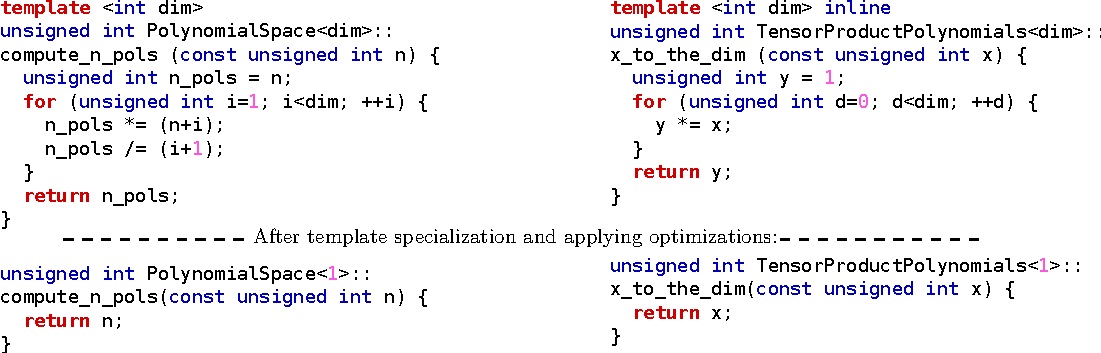
\includegraphics[width=0.95\linewidth]{figs/identical-example.pdf}
%  \caption{Two function extracted from the 447.dealII benchmark that are not
%           identical at the source level, but after applying template
%           specialization and optimizations they become identical at the IR
%           level.}
%  \label{fig:identical-example}
%\end{figure*}


\subsection{Compilation Overhead}

\begin{figure*}[t]
  \centering
  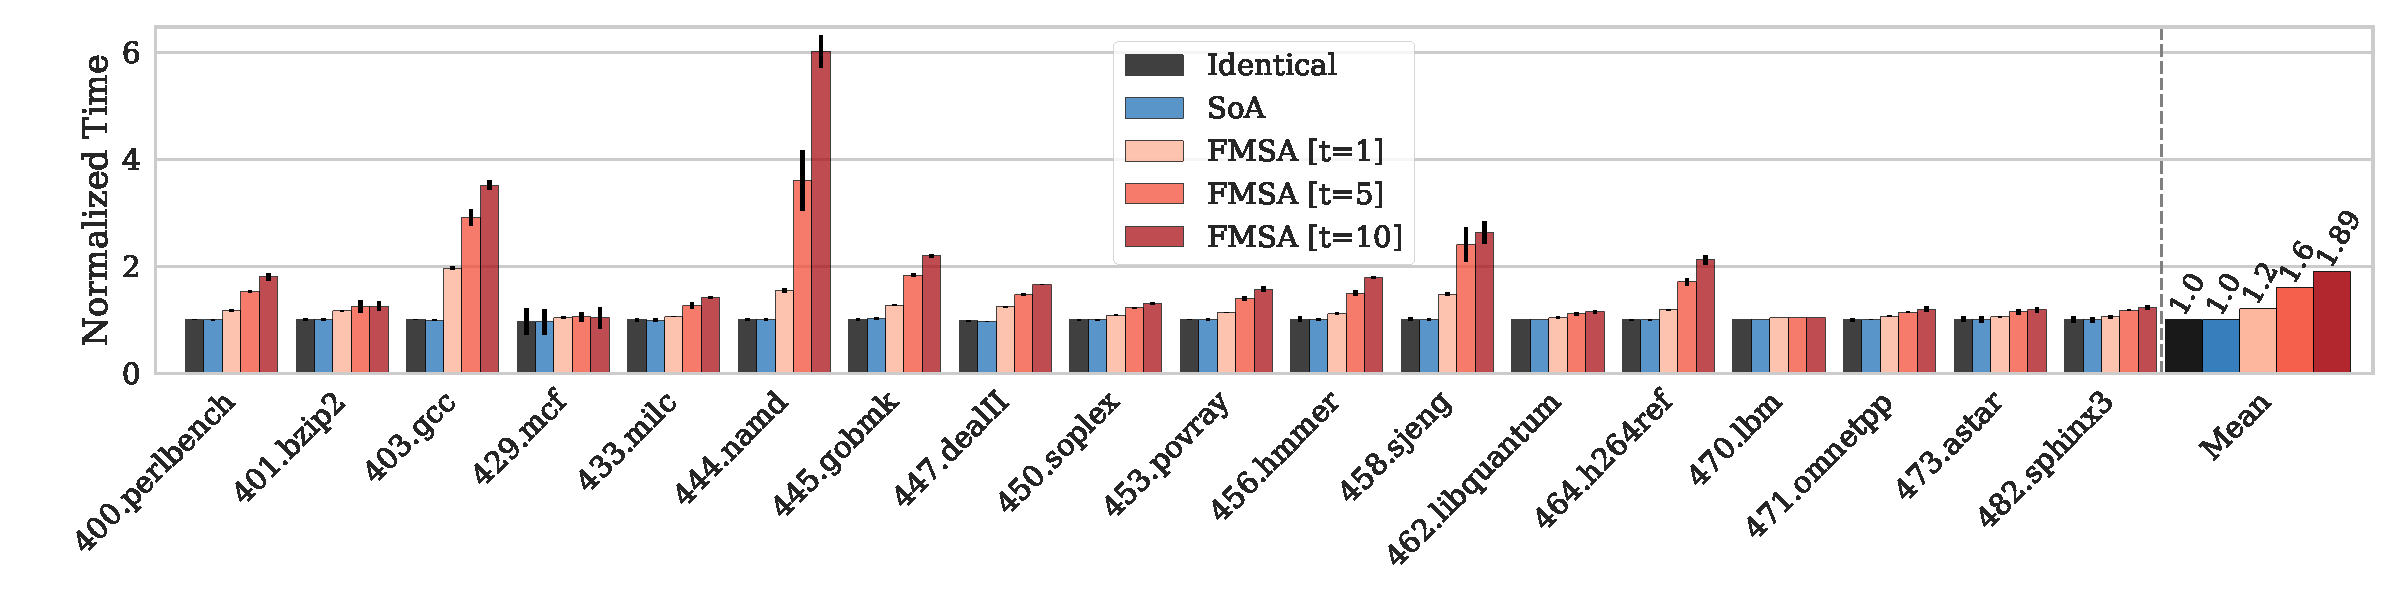
\includegraphics[width=\linewidth]{figs/compilation-time.pdf}
  \vspace{-4ex}
	\caption{Compilation-time overhead on the Intel platform. For exhaustive exploration (not shown) the average overhead is 25$\times$. Through ranking, we reduce overhead by orders of magnitude. For an exploration threshold of one, FMSA has an overhead of only 20\%.}
  \label{fig:compilation-time}
\end{figure*}


Figure~\ref{fig:compilation-time} shows the compilation-time overhead for all optimizations. As explained in the experimental setup, we
only present results when compiling for the Intel platform. Since we cross-compile on the same machine for both targets, compilation times
are very similar. We also do not include results for the oracle (exhaustive) exploration. It would be hard to visualize it in the same plot
as the other configurations, since it can be up to 136$\times$ slower than the baseline.

\begin{figure}[t]
  \centering
  %\hspace{-2ex}
  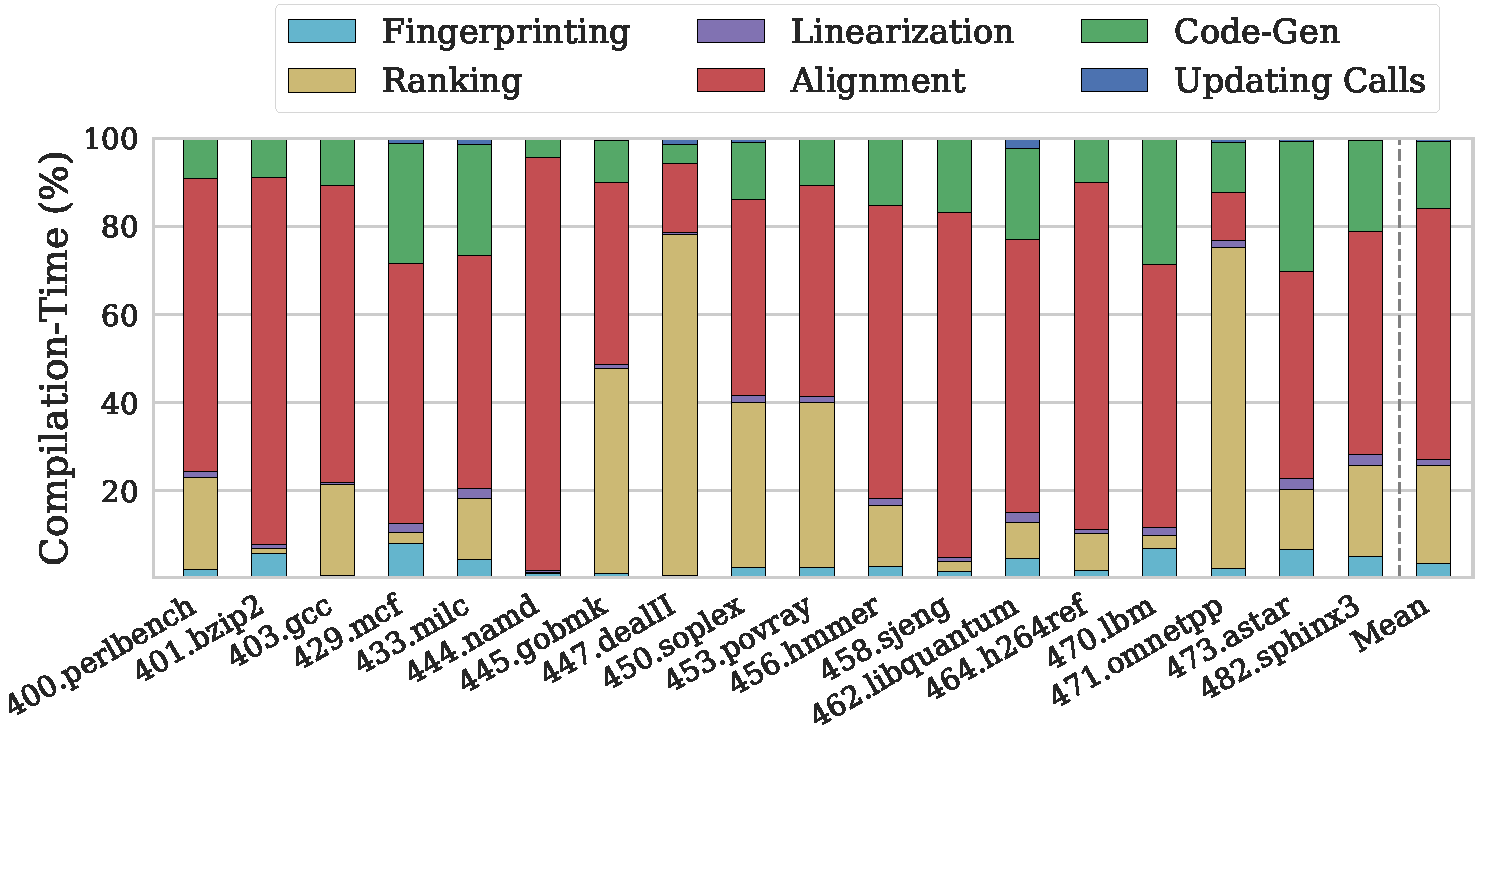
\includegraphics[width=1.0\linewidth]{figs/compilation-time-breakdown-sqrd.pdf}
  \vspace{-8.5ex}
  \caption{A compilation-time breakdown isolating the percentage for each major
           step of the optimization (t=1).}%, with an exploration threshold of one.}
  \label{fig:compilation-time-breakdown}
\end{figure}

\begin{figure*}[t]
  \centering
  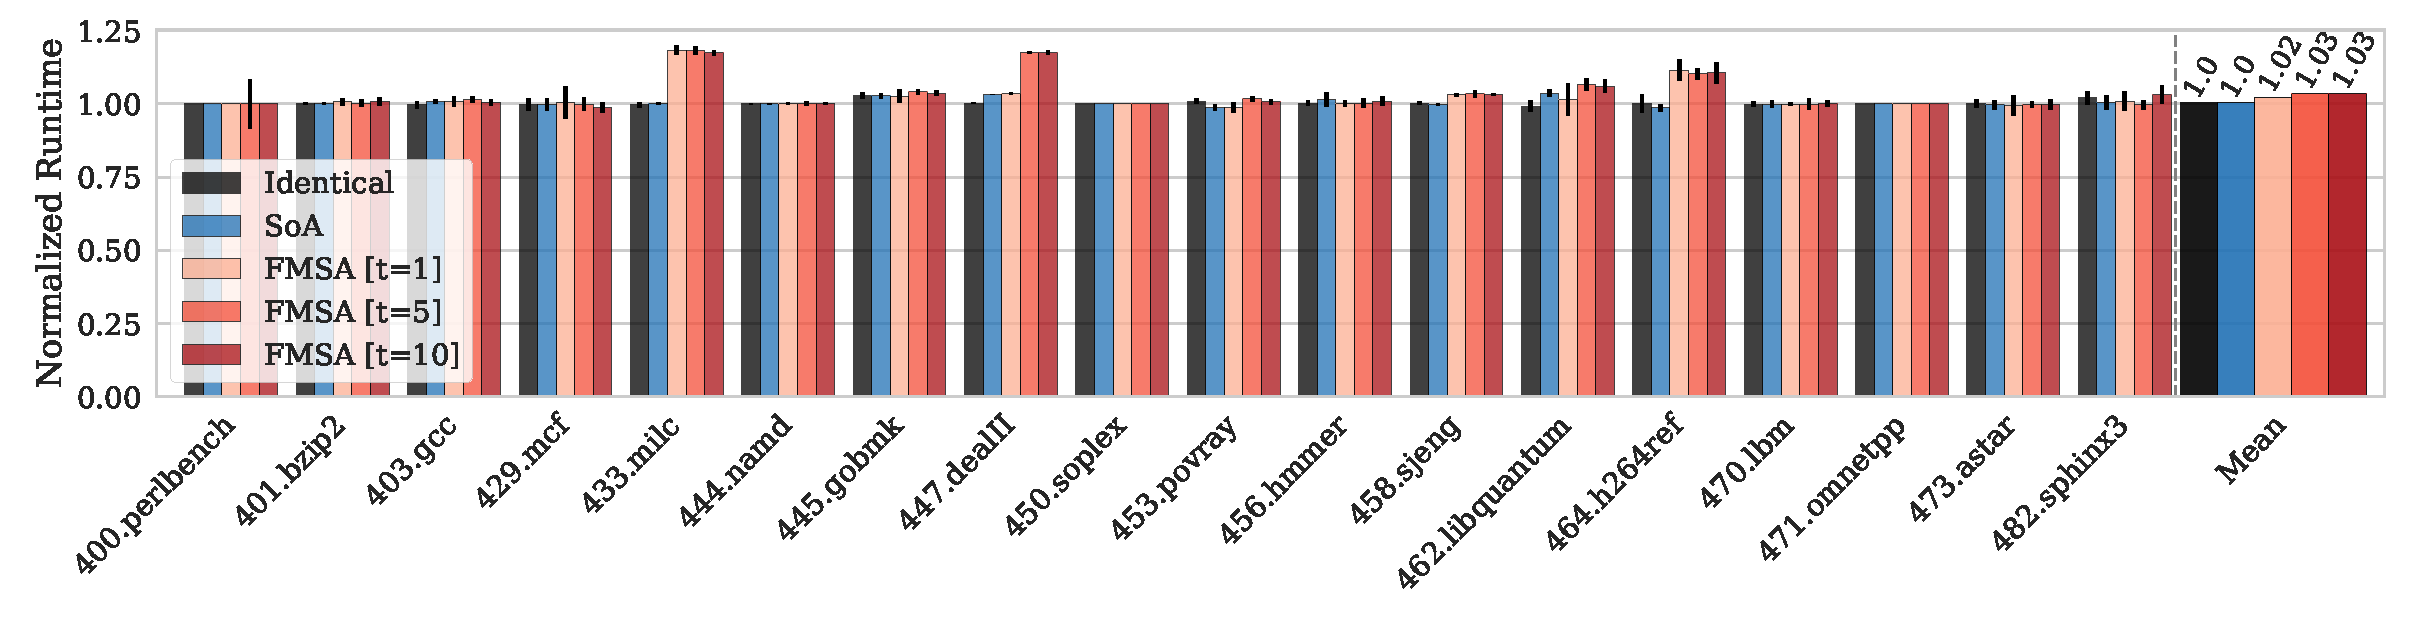
\includegraphics[width=\linewidth]{figs/runtime-impact.pdf}
  \vspace{-4ex}
	\caption{Runtime overhead on the Intel platform. Performance impact is almost always statistically insignificant. For the few benchmarks affected, FMSA merges hot functions.}
  \label{fig:runtime-impact}
\end{figure*}

Unlike the other evaluated techniques, our optimization is a prototype implementation, not yet tuned for compilation-time. We believe that
compilation-time can be further reduced with some additional engineering effort. Nevertheless, by using our ranking infrastructure to
target only the single most promising equivalent function for each function we examine, we reduce compilation-time overhead by up to two
orders of magnitude compared to the oracle. This brings the average compile-time overhead to only 20\% compared to the baseline, while
still reducing code size almost as well as the oracle. Depending on the acceptable trade-off between compilation-time overhead and code
size, the developer can change the exploration threshold to exploit more opportunities for code reduction, or to accelerate compilation.

Figure~\ref{fig:compilation-time-breakdown} shows a detailed compilation-time breakdown. For each major step of the proposed optimization,
we present the accumulated time spent across the whole program. To better understand the overhead of each one of the steps, we use an
exploration threshold of one ($t = 1$). Because the ranking mechanism performs a quadratic operation on the number of functions, computing
the similarity between all pairs of functions, it is expected that ranking would be amongst the most costly steps. However, it is
interesting to notice that the sequence alignment dominates most of the compilation-time overhead, especially considering that this
operation is performed only once per function, when $t = 1$. Although this operation is linear on the number of functions, the
Needleman-Wunsh algorithm~\cite{needleman70} is quadratic on the size of the functions being aligned, both in time and space.
Unsurprisingly, code generation is the third most costly step, which also includes the time to optimize the merge of the parameters. The
remaining steps contribute, in total, a small percentage of all the compilation-time overhead. This analysis suggests that optimizing the
sequence alignment algorithm and the ranking mechanism is key to reducing even further the overall compilation-time overhead.

%\vspace{-1ex}
\subsection{Performance Impact}


The primary goal of function merging is to reduce code size. Nevertheless, it is also important to understand its impact on the programs'
execution time and the trade-offs between performance and code size reduction. Figure~\ref{fig:runtime-impact} shows the normalized
execution time. Overall, our optimization has an average impact of about 3\% on programs' runtime. For most benchmarks, there is no
statistically significant difference between the baseline and the optimized binary. Only for \texttt{433.milc}, \texttt{447.dealII}, and
\texttt{464.h264ref} there is a noticeable performance impact.

We take \texttt{433.milc}, which has the worst result, for discussion. For an exploration threshold value of one, we merge 58 functions for this
benchmark. Through profiling, we discovered that a handful of them contain hot code, that is, they have basic blocks that are frequently executed. If we prevent these hot
functions from merging, all performance impact is removed while still reducing code size. Specifically, our original results showed a
5.11\% code size reduction and an 18\% performance overhead.
%%RODRIGO: The performance impact goes actually to zero (no statistical difference)
By avoiding merging hot functions, it results in effectively non-existent performance impact and
a code size reduction of 2.09\%.
%%RODRIGO: 9$\times$ is wrong. 18\% is performance overhead; 2.09\% is code reduction; the previous code reduction was 5.11\%.
This code size reduction is still about twice as good as the state-of-the-art. As with the
compilation overhead, this is a trade-off that the developer can control.

%Note that the state-of-the-art has a reduction of only 1.09\% on this benchmark.
%If we can be more permissive, allowing some of the hot functions to be merged,
%we can have a code size reduction of 3.43\% while keeping the performance impact
%at about 4\%.

%However, \text{quantum\_gate1} is the largest function in the program,
%which means that this merge operation greatly contributes
%to the overall code-size reduction.
%Preventing this merge results in the code-size reduction dropping from 16\% to
%6.9\%, which is still a very significant code-size reduction compared to the
%other techniques that show no reduction on this particular benchmark.

%It is interesting to note that, for the 447.dealII benchmark, FMSA [t=1] has
%no extra impact than the state-of-the-art


%As a case study, we analyze the performance impact on the \text{462.libquantum}
%benchmark.
%After a detailed inspection of the program's execution with profiling
%information, we identified only two functions that contain the hottest basic
%blocks in the whole program.
%Hot basic blocks are determined based on the block frequencies recorded by
%instrumenting all basic blocks in the program~\cite{ball94}.
%The two hottest functions are: \text{quantum\_gate1} and
%\text{quantum\_decohere}.
%If we cross this information with the list of merged functions, we can confirm
%that the function \text{quantum\_gate1} is involved in a merge operation with
%a non-identical function.

%If, instead, we prevent this function of being merged, the performance
%impact goes away and we end up with a performance which is statistically
%equivalent to the baseline version.
%However, \text{quantum\_gate1} is the largest function in the program,
%which means that this merge operation greatly contributes
%to the overall code-size reduction.
%Preventing this merge results in the code-size reduction dropping from 16\% to
%6.9\%, which is still a very significant code-size reduction compared to the
%other techniques that show no reduction on this particular benchmark.

\vspace{-2ex}
\section{Related Work}

Throughout the years, there have been increasing efforts towards code-size
optimizations.
%Most of the classic optimizations try to find semantically equivalent programs
%that require fewer instructions to execute, such as dead code elimination,
%common subexpression elimination, and others~\cite{cocke70,massalin87,knoop94}.
Compiler optimizations for code-size reduction exist since the very begining
of optimizing compilers.
These optimizations can be divided in two main categories:
those that replace a piece of code by a smaller but semantically equivalent code,
changing the instructions and operations performed~\cite{massalin87,tanenbaum82};
and those that remove or combine redundant code~\cite{cocke70,knoop94,ernst97,
                                              cooper99,debray00,chen03,loki04}.
One optimization from this second category is function
merging.

Google developed an optimization for the \textit{gold} linker that merges
identical functions on a bit-level~\cite{tallam10,kwan12}.
After placing each function in a separate ELF section, they identify function
sections that have their \textit{text} section bit-identical and also their
relocations point to identical sections.
%A simpler version of this optimization was also offered by the MSVC linker~\cite{msvc-icf};
A similar optimization for merging identical functions %, but implemented at the IR level,
is also offered by both GCC and LLVM~\cite{llvm-fm,livska14}.
In Section~\ref{sec:background}, we presented a detailed description of the
related work on function-merging, including the state-of-the-art~\cite{edler14}.


%\subsection{Code Factoring}

%Function merging and code factoring are different techniques for solving the
%same fundamental problem of duplicated code.
Code factoring is a different technique for solving the same fundamental problem
of duplicated code.
%While the former works by merging similar functions, the latter works by
%factoring out duplicated code~\cite{loki04}.
%Instead of merging similar functions, code factoring works by factoring out
%duplicated code into separate functions~\cite{loki04}.
Code factoring can be applied at different levels of the program~\cite{loki04}.
Local factoring, also known as local code motion, moves identical instructions
from multiple basic blocks to either their common predecessor or successor,
whenever valid~\cite{knoop94,briggs94,loki04}.
Procedural abstraction (or outlining) finds identical code
that can be extracted into a separate function, replacing all replicated
occurrences with a function call~\cite{loki04,dreweke07}.

Procedural abstraction differs from function merging as it usually works on
single basic blocks or single-entry single-exit regions.
Moreover, it only works for identical segments of code, and every identical
segment of code is extracted into a separately new function.
Function merging, on the other hand, works on whole functions, which can be
identical or just partially similar, producing a single merged function.

However, all these techniques are orthogonal to the proposed optimization and
could complement each other at different stages of the compilation pipeline.

\vspace{-1ex}
\section{Conclusion}

We have presented a novel technique, based on sequence alignment, for merging
functions that addresses major limitations of the existing solutions.
We have also proposed a ranking-based exploration mechanism so that we can focus
the optimization on promising pairs of functions, reducing considerably the
compilation-time overhead, compared to the oracle's quadratic exploration.
With this framework, our prototype introduces an average
compilation-time overhead of only 20\%.
Our optimization shows code-size reductions up to 22\%, with an overall average
of about 5.6\%.
This optimization can be carried on without any significant impact on
performance when profiling information is used.

%Allowed instruction reordering could be performed in order to improve coverage
%of the proposed function merging strategy.
%Although we perform sequence alignment directly on the functions after
%linearization, some functions can have their instructions reodered without
%changing their semantics.
%This instruction reodering could potentially improve the alignment of two given
%functions.
%However, it is a constly operation that can significantly degrade compilation
%time.

For future work, we plan to focus on improving the ranking mechanism to reduce
compilation time even further.
A better compilation time can also be achieved by integrating the
function-merging optimization to a summary-based parallel link-time optimization
framework, such as ThinLTO in LLVM.
We also plan to work on the linearization of the candidate functions, allowing
instruction reordering to maximize the number of matches between the functions.
%Have a linearization of the candidates based on the current function:
%Lin(F1) = canonical linearization of F1, then linearize F2 based on Lin(F1).




%% Leave some space for the Acknowledgments, that I (Rodrigo) am required to mention.
%% \section*{Acknowledgments}
%% This work was supported blah blah.

%% Acknowledgments, if needed.

% We recommend abbrvnat bibliography style.

\bibliographystyle{abbrvnat}


% The bibliography should be embedded for final submission.

%% \begin{thebibliography}{}
%% \softraggedright

%% \bibitem[Smith et~al.(2009)Smith, Jones]{smith02}
%% P. Q. Smith, and X. Y. Jones. ...reference text...

\bibliography{bib/refs.bib}
%% \end{thebibliography}


\end{document}
